\documentclass[11pt]{article}
\usepackage[utf8]{inputenc}
\usepackage[spanish]{babel}
\decimalpoint
\usepackage{amsmath}
\usepackage{amsthm}
\usepackage{amssymb}
\usepackage{graphicx}
\usepackage[margin=0.8in]{geometry}
\usepackage{fancyhdr}
\usepackage[inline]{enumitem}
\usepackage{float}
\usepackage{cancel}
\usepackage{bigints}
\usepackage{listings}
\usepackage{xcolor}
\usepackage{listingsutf8}
\usepackage{algpseudocode}
\usepackage{algorithm}
\usepackage{apacite}
\usepackage{tcolorbox}
\usepackage{multicol}
\usepackage{tipa}
\usepackage{caption} 
\pagestyle{fancy}
\usepackage{hyperref}
\usepackage{mathtools}% http://ctan.org/pkg/mathtools

\hypersetup{
    colorlinks,
    citecolor=black,
    filecolor=black,
    linkcolor=black,
    urlcolor=black
}
\newcommand{\xvdash}[1]{%
	\vdash^{\mkern-10mu\scriptscriptstyle\rule[-.9ex]{0pt}{0pt}#1}%
}
\setlength{\headheight}{15pt} 
\lhead{Tarea 4. Chat multicast}
\rhead{\thepage}
\lfoot{ESCOM-IPN}
\renewcommand{\footrulewidth}{0.5pt}
\setlength{\parskip}{0.5em}
\newcommand{\ve}[1]{\overrightarrow{#1}}
\newcommand{\abs}[1]{\left\lvert #1 \right\lvert}
\newcommand{\blank}{\text{\textcrb}}
\date{\today}
\title{Tarea 4. Chat multicast}
\author{Sanchez Mendez Edmundo Josue}

\bibliographystyle{apacite}
\begin{document}
		\begin{titlepage}
			\begin{center}
				
				% Upper part of the page. The '~' is needed because \\
				% only works if a paragraph has started.
				
				\noindent
				\begin{minipage}{0.5\textwidth}
					\begin{flushleft} \large
						
\includegraphics[width=0.5\textwidth]{resources/ipn.png}
					\end{flushleft}
				\end{minipage}%
				\begin{minipage}{0.55\textwidth}
					\begin{flushright} \large
						
\includegraphics[width=0.5\textwidth]{resources/escom.png}
					\end{flushright}
				\end{minipage}
				
				\textsc{\LARGE Instituto Politécnico Nacional}\\[0.5cm]
				
				\textsc{\Large Escuela Superior de Cómputo}\\[1cm]
				
				% Title
				
				{ \huge Tarea 4. Chat multicast \\[1cm] }
				
				{ \Large Unidad de aprendizaje: Desarrollo de Sistemas Distribuidos} \\[1cm]
				
				{ \Large Grupo: 4CV11 } \\[1cm]
				
				\noindent
				\begin{minipage}{0.5\textwidth}
					\begin{flushleft} \large
						\emph{Alumno:} \\
						Sanchez Mendez Edmundo Josue
					\end{flushleft}
				\end{minipage}%
				\begin{minipage}{0.5\textwidth}
					\begin{flushright} \large
						\emph{Profesor:} \\
						Pineda Guerrero Carlos 
					\end{flushright}
				\end{minipage}
				
				\vfill
				% Bottom of the page
				{\large {\today}}
			\end{center}
		\end{titlepage}
	
	\titlepage
	\tableofcontents
	\newpage
	
	\section{Introducción}
		Mediante el desarrollo de un solo programa en Java en modo consola se implementara un chat utilizando comunicación multicast mediante datagramas. Se deberá ejecutar el programa en una máquina virtual con Windows Server 2012 en Azure. El funcionamiento general del programa es el siguiente:
		\begin{itemize}
			\item El programa creará un thread que actuará como cliente multicast, el cual recibirá los mensajes del resto de los nodos. Cada mensaje recibido será desplegado en la pantalla. El thread desplegará el mensaje que envía el mismo nodo.
			\item En el método main(), dentro de un ciclo infinito:
			\begin{itemize}
				\item Se desplegará el siguiente prompt: ``Ingrese el mensaje a enviar: '' (sin las comillas), entonces se leerá una string (el mensaje).
				\item Se deberá enviar el mensaje a los nodos que pertenecen al grupo identificado por la IP 230.0.0.0 a través del puerto 10000. El paquete a enviar deberá tener la siguiente forma: nombre\_usuario:mensaje\_ingresado dónde nombre\_usuario es el nombre del usuario que pasó como parámetro al programa (hugo, paco o luis) y mensaje\_ingresado el mensaje que el usuario ingresó por el teclado, separados por el carácter ``:'' sin espacios.
			\end{itemize}
		\end{itemize}

	\section{Desarrollo}
El desarrollo de esta tarea no fue nada complicada, ya que habíamos hecho un ejercicio similar en clase y prácticamente fue solo implementar el código visto, sin embargo, una de las cosas más interesantes fue el cómo imprimir lo signos de interrogación y las letras acentuadas en CMD, esto fue un gran conflicto ya que Windows puede usar diferentes páginas de códigos, estas páginas nos define el conjunto de caracteres que se está utilizando, usualmente Windows tiene por defecto la pagina 850, 437 o la 1252, las cuales son diferentes en cuanto a codificación de los caracteres, para poder saber que numero de página utiliza nuestro CMD se usa el comando: chcp, para cambiarlo usamos chcp n, donde n es el número de página.\par
La página 437 que Java reconoce como IBM437, la cual es usada en la región de los Estados Unidos, esta página es el conjunto de caracteres que incorporaba la primera versión del Personal Computer (PC) de IBM, hay pequeñas diferencias con las otras dos páginas de códigos que usa Windows, de hecho, las otras dos se crearon para poder complementar esta página.\par
La página 850 fue creada para varios idiomas por lo que se le llama Multilingual (Latin I) a veces denominada Europa occidental, esta página a diferencia de la página 4337 es que varios caracteres empleados para el dibujo de cuadros, así como letras griegas y otros fueron reemplazados por caracteres latinos con diacríticos requeridos por idiomas como el español, Java la reconoce como IBM850.\par
Por último, la pagina 1252 que Java reconoce como windows-1252	 es una codificación de caracteres del alfabeto latino, usada por defecto cuando unicode no se usa en los componentes oficiales de Microsoft Windows en inglés y en algunos lenguajes occidentales. Esta codificación es un superconjunto de ISO 8859-1 \par
Ahora el desarrollo de la práctica se hizo en mi laptop la cual usa la pagina 850, esta página tiene los caracteres especiales que se usaran en las pruebas de esta práctica. Ahora al querer usar esta pagina al insertar el carácter ``¿'' el resultado al mandar el mensaje era el carácter “ lo cual es erróneo, al empezar el desarrollo de la práctica lo cual fue hace unos días me di cuenta de que si usamos la pagina 1252 y usamos UTF-8 esto era solucionado y la impresión era correcta, como podemos ver en la figura 1, esto lo logre ya que decidí ver como se codificaban los caracteres que ingresaba el chat, las lineas de código están comentadas.	
		\begin{figure}[H]
			\centering
			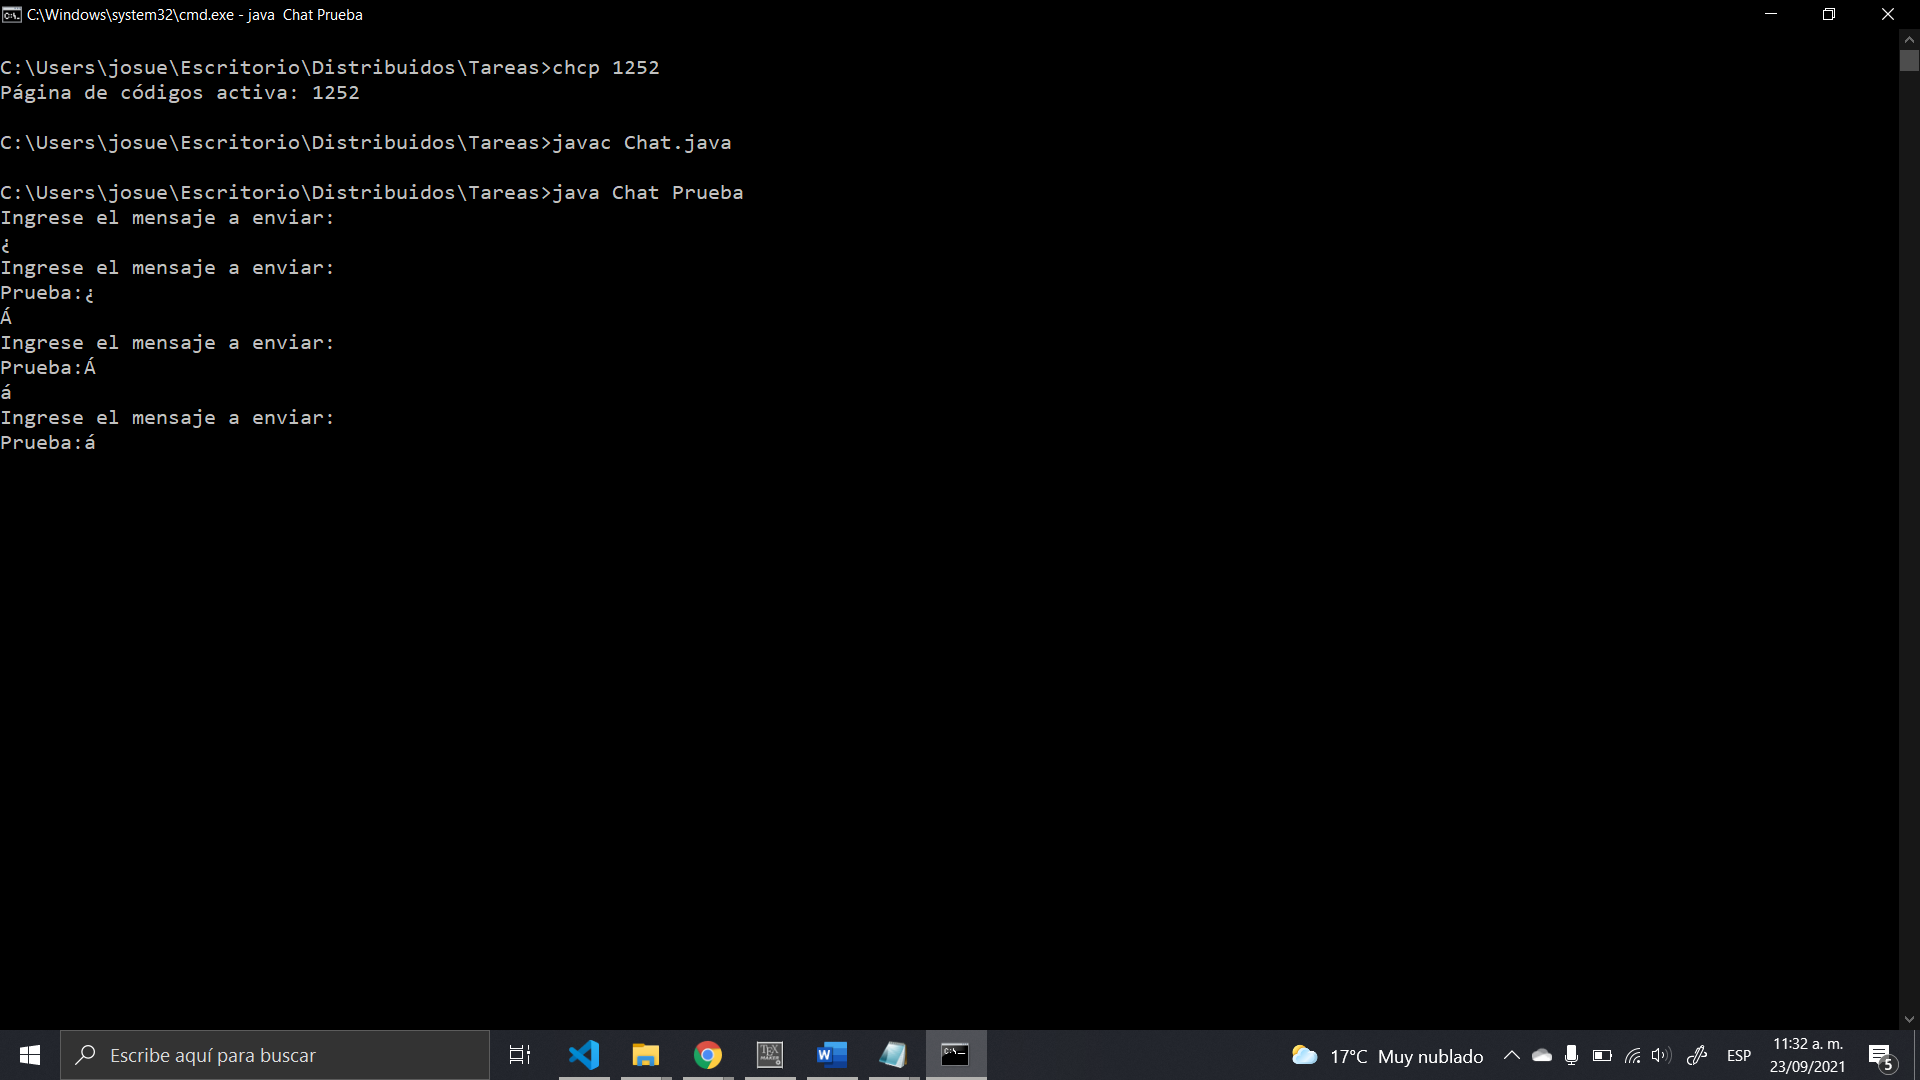
\includegraphics[scale=0.43]{resources/prueba1252utf8.png}
			\caption{Prueba usando la página 1252 y UTF-8.}\label{fig:picture}
		\end{figure}		
Ahora me doy cuenta de que estaba cometiendo un error, lo mas adecuado era adaptarse a la pagina en uso de nuestro CMD ya que, como veremos mas adelante en el reporte podrían surgir errores al momento de ejecutar el programa en nuestra máquina virtual.\par
Por lo que para poder usar la pagina por defecto de mi computadora la cual es la 850, no solo era necesario poner que tipo de codificación se usuaria al momento de desplegar el mensaje enviado en el chat o al momento de enviar el mensaje de forma multicast, sino que también al momento de leer el mensaje desde la consola, en mi caso uso Scanner, por lo que también se le tenia que colocar el tipo de decodificación, como estamos usando la pagina 850 el nombre que reconoce Java es IBM850, y así como vemos en la figura 2 el programa funciona correctamente.\par 
		\begin{figure}[H]
			\centering
			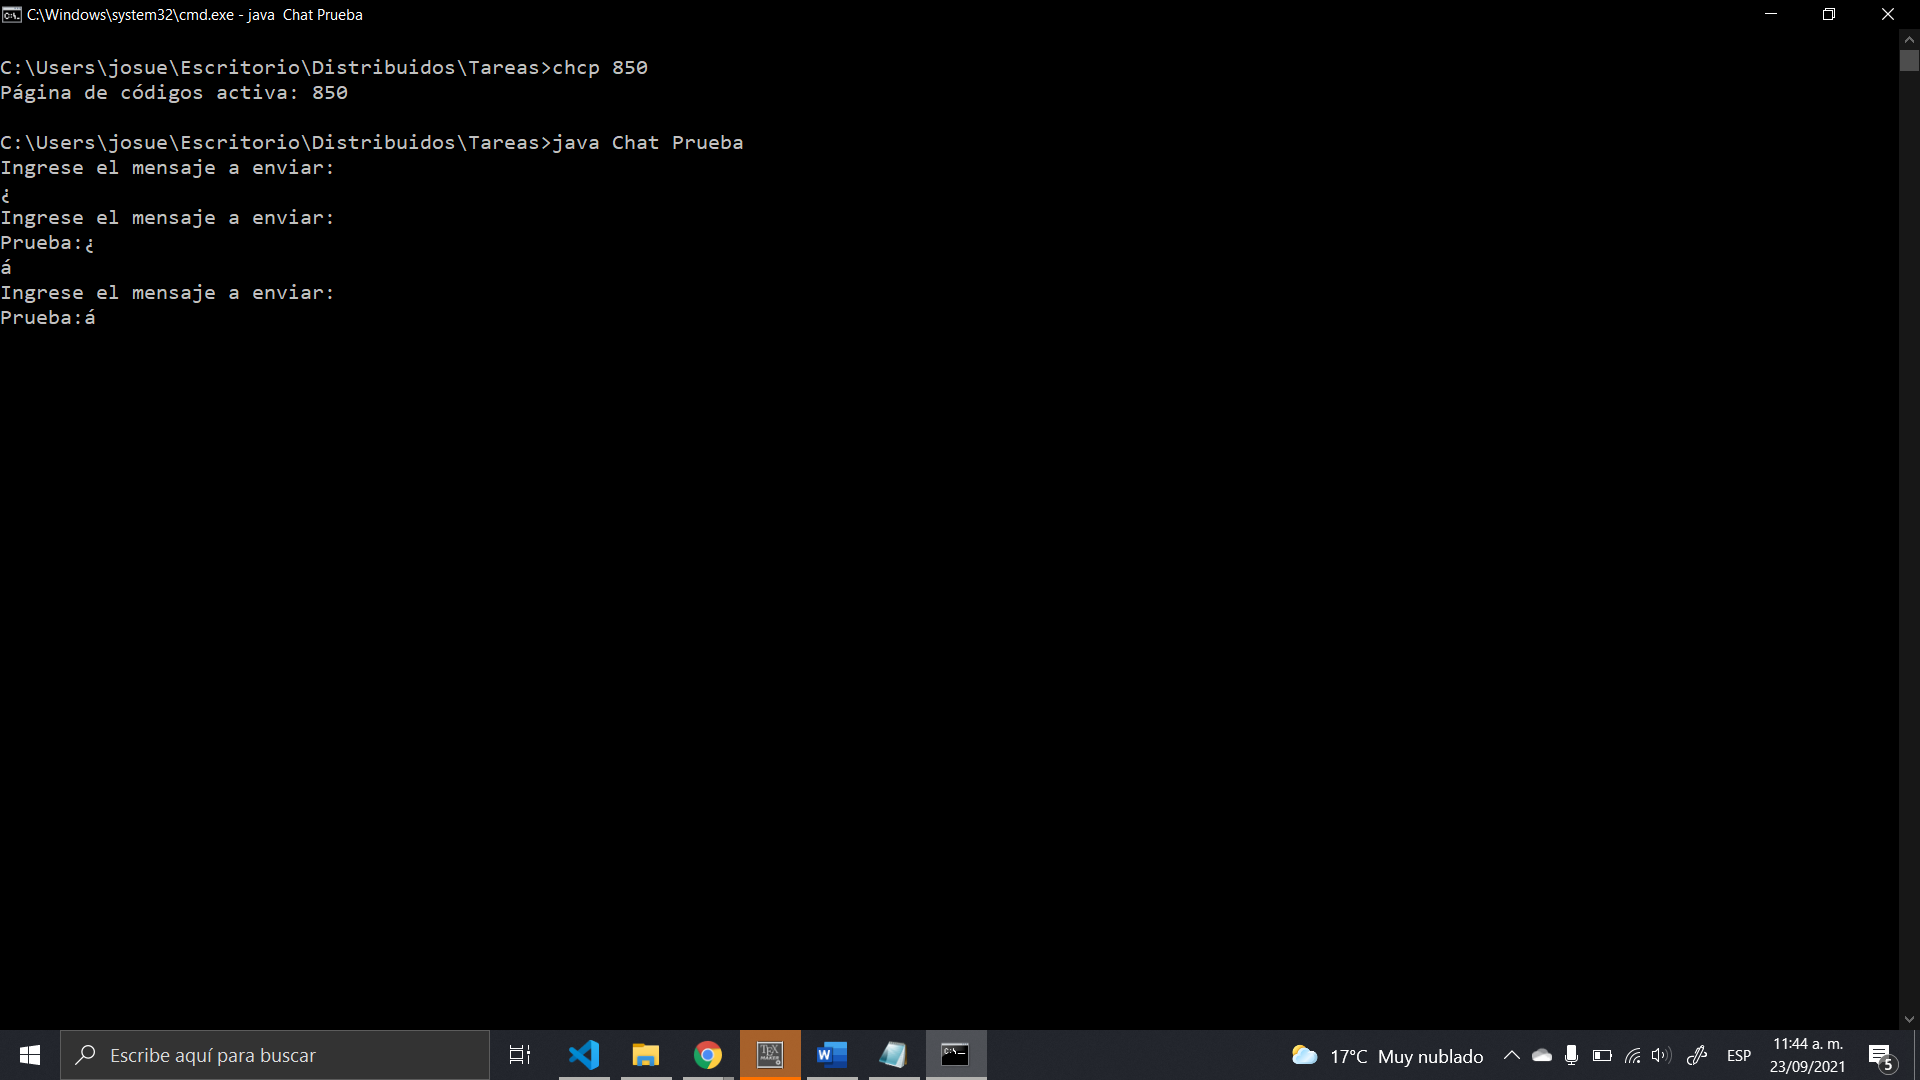
\includegraphics[scale=0.43]{resources/prueba850ibm.png}
			\caption{Prueba usando la página 850 e IBM850.}\label{fig:picture}
		\end{figure}
Para llegar a lo anterior tuve que pasar por varias pruebas y básicamente por el método del ensayo y error, de hecho la solucion a este problema cuando estaba probando el programa en la maquina virtual. Me tarde poco mas de 4 horas en total para poder solucionar este problema, la ventaja fue que el costo de la maquina virtual era de menos de 1 peso por hora de uso por lo que si comparamos los casi 4 pesos que se usaron para esta practica contra los 100 dolares que nos da el correo institucional es casi nada.\par

Ahora el siguiente punto interesante fue como recibir el mensaje que escribirá el usuario, a través de mi experiencia de trabajo con Java solo vi 2 alternativas, usar Scanner o usar BufferedReader, por lo que se y recuerdo Scanner hace lo mismo que BufferedReader al mismo nivel con la misma eficiencia, sin embargo, Scanner tiene muchas funciones mas pero el cambio o la diferencia que considero mas importante es el tamaño del buffer y es que BufferedReader tiene un tamaño de 8192 caracteres en comparación del Scanner tiene solo 1024 caracteres en el buffer, al ver eso considero mejor usar Scanner ya que al ser un chat y con base a las pruebas a realizar es mas que suficiente para este caso. Ahora si vemos el condigo dado para recibir mensajes necesitamos una longitud del mensaje, lo usual seria usar el mismo tamaño del buffer de Scanner, sin embargo, para estas pruebas seria contraproducente ya que ningún mensaje a enviar tiene esa longitud y esto provocaría que se impriman caracteres vacíos, en mi opinión lo mejor es ajustar el tamaño con base a los requerimientos de la practica, ademas de que al momento de las pruebas el chat se vera mejor, por lo que el valor a usar sera 50 ya que es el tamaño suficiente para la prueba, en caso de querer enviar mensajes mas largos se tendrá que cambiar la variable BUFSIZ a lo que se necesite pero como valor máximo 1024 ya que si ponemos un valor mas grande leeremos los 1024 y los caracteres restantes no se imprimirán, en caso de que necesitemos enviar mensajes mas grandes tendríamos cambiar la forma de lectura en consola.\par

\subsection{Configuración de maquina virtual}
Ahora vayamos a la creación de la maquina virtual la cual tendrá que tener las siguientes características.
		\begin{itemize}
			\item SO: Windows Server 2012.
			\item Nombre de la maquina virtual: W2019630428    
		\end{itemize}
		\begin{figure}[H]
			\centering
			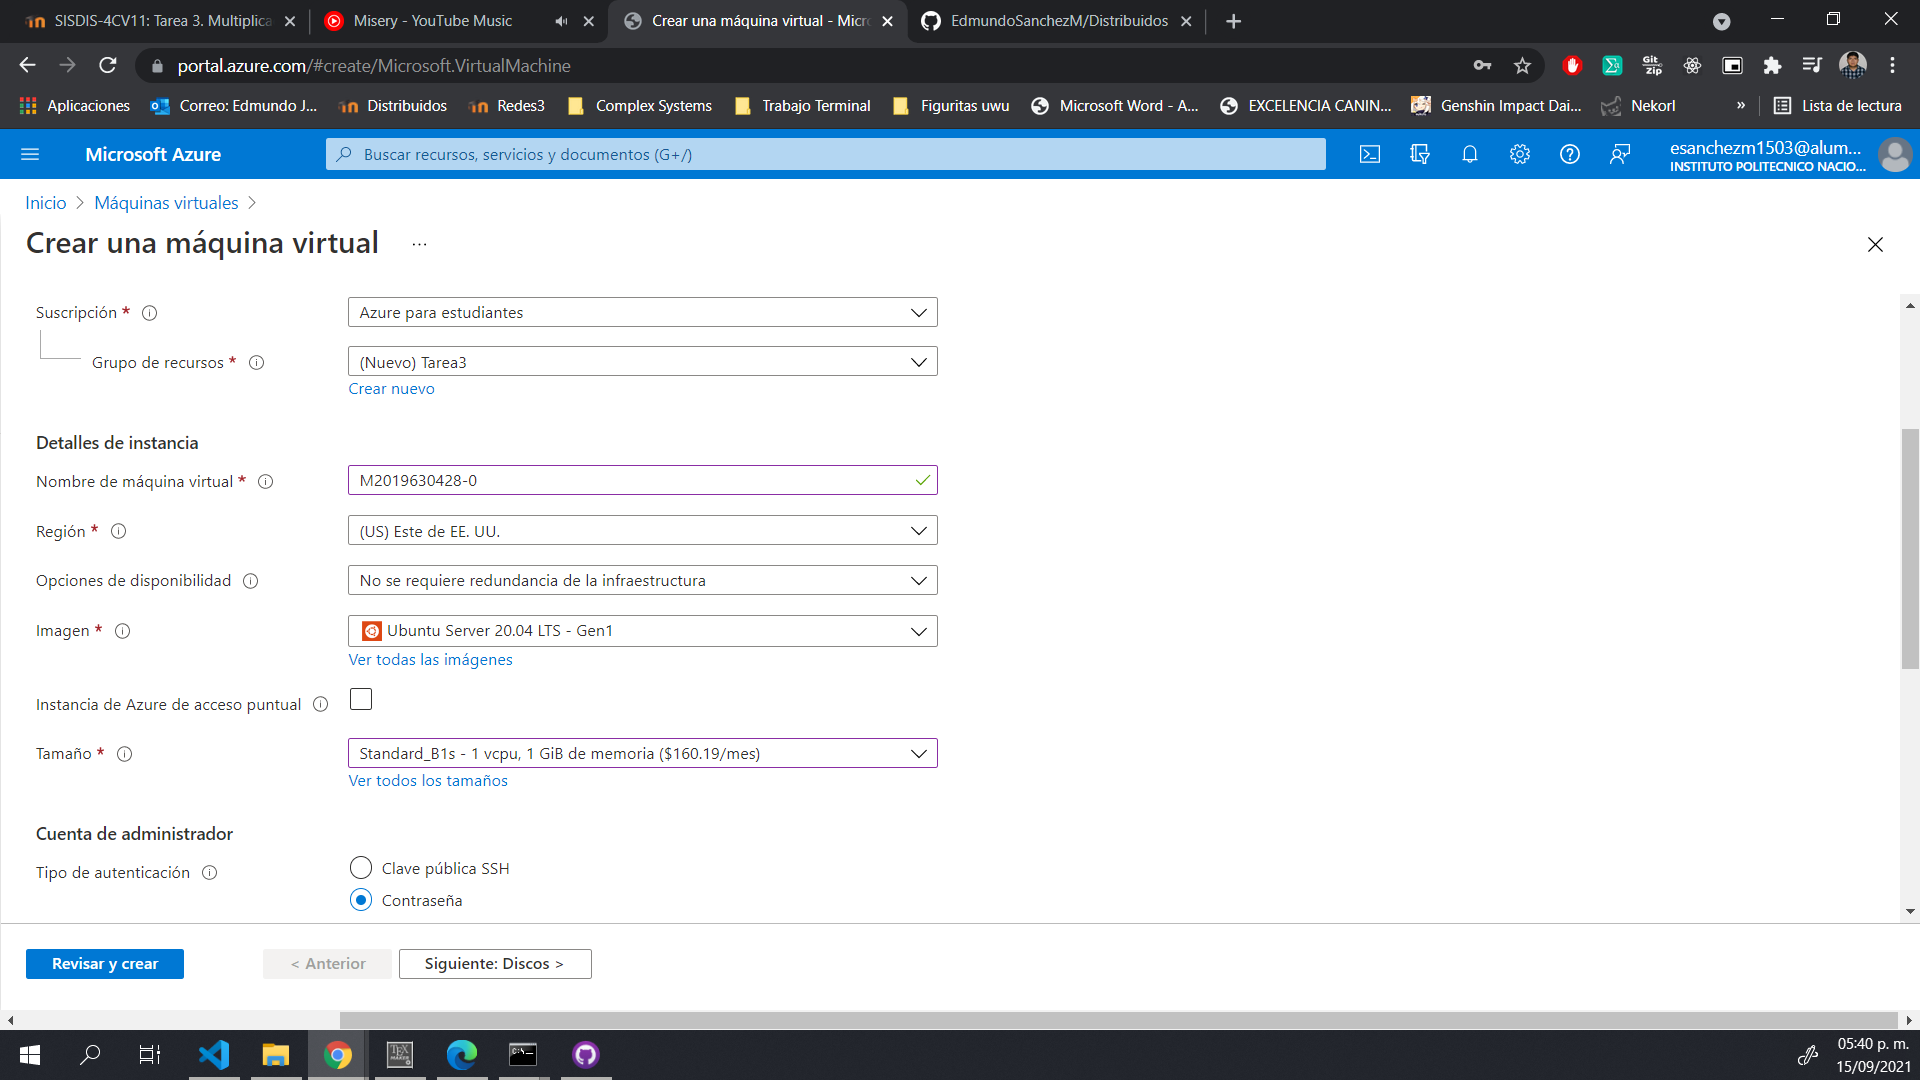
\includegraphics[scale=0.34]{resources/datosbasicos.png}
			\caption{Información básica. }\label{fig:picture}
		\end{figure}
		\begin{figure}[H]
			\centering
			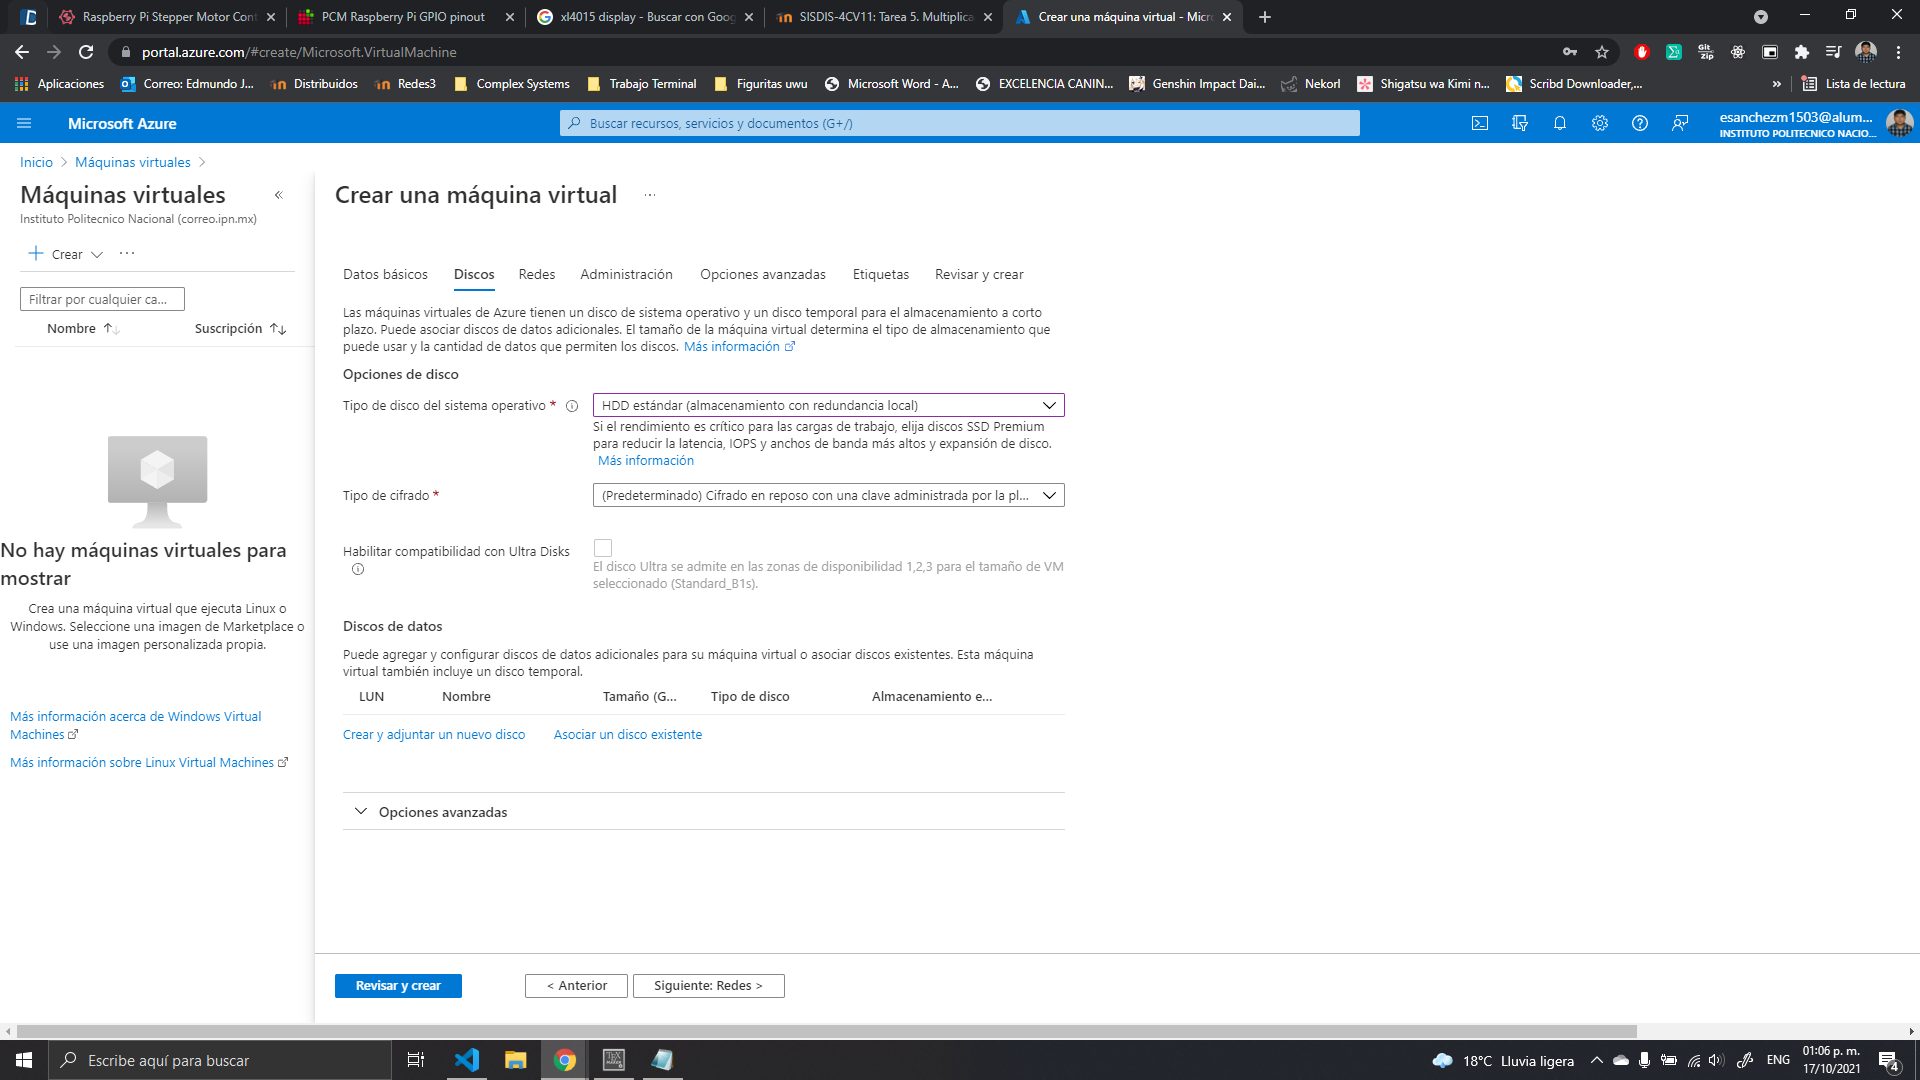
\includegraphics[scale=0.34]{resources/datosdisco.png}
			\caption{Configuración del tipo de disco. }\label{fig:picture}
		\end{figure}
		\begin{figure}[H]
			\centering
			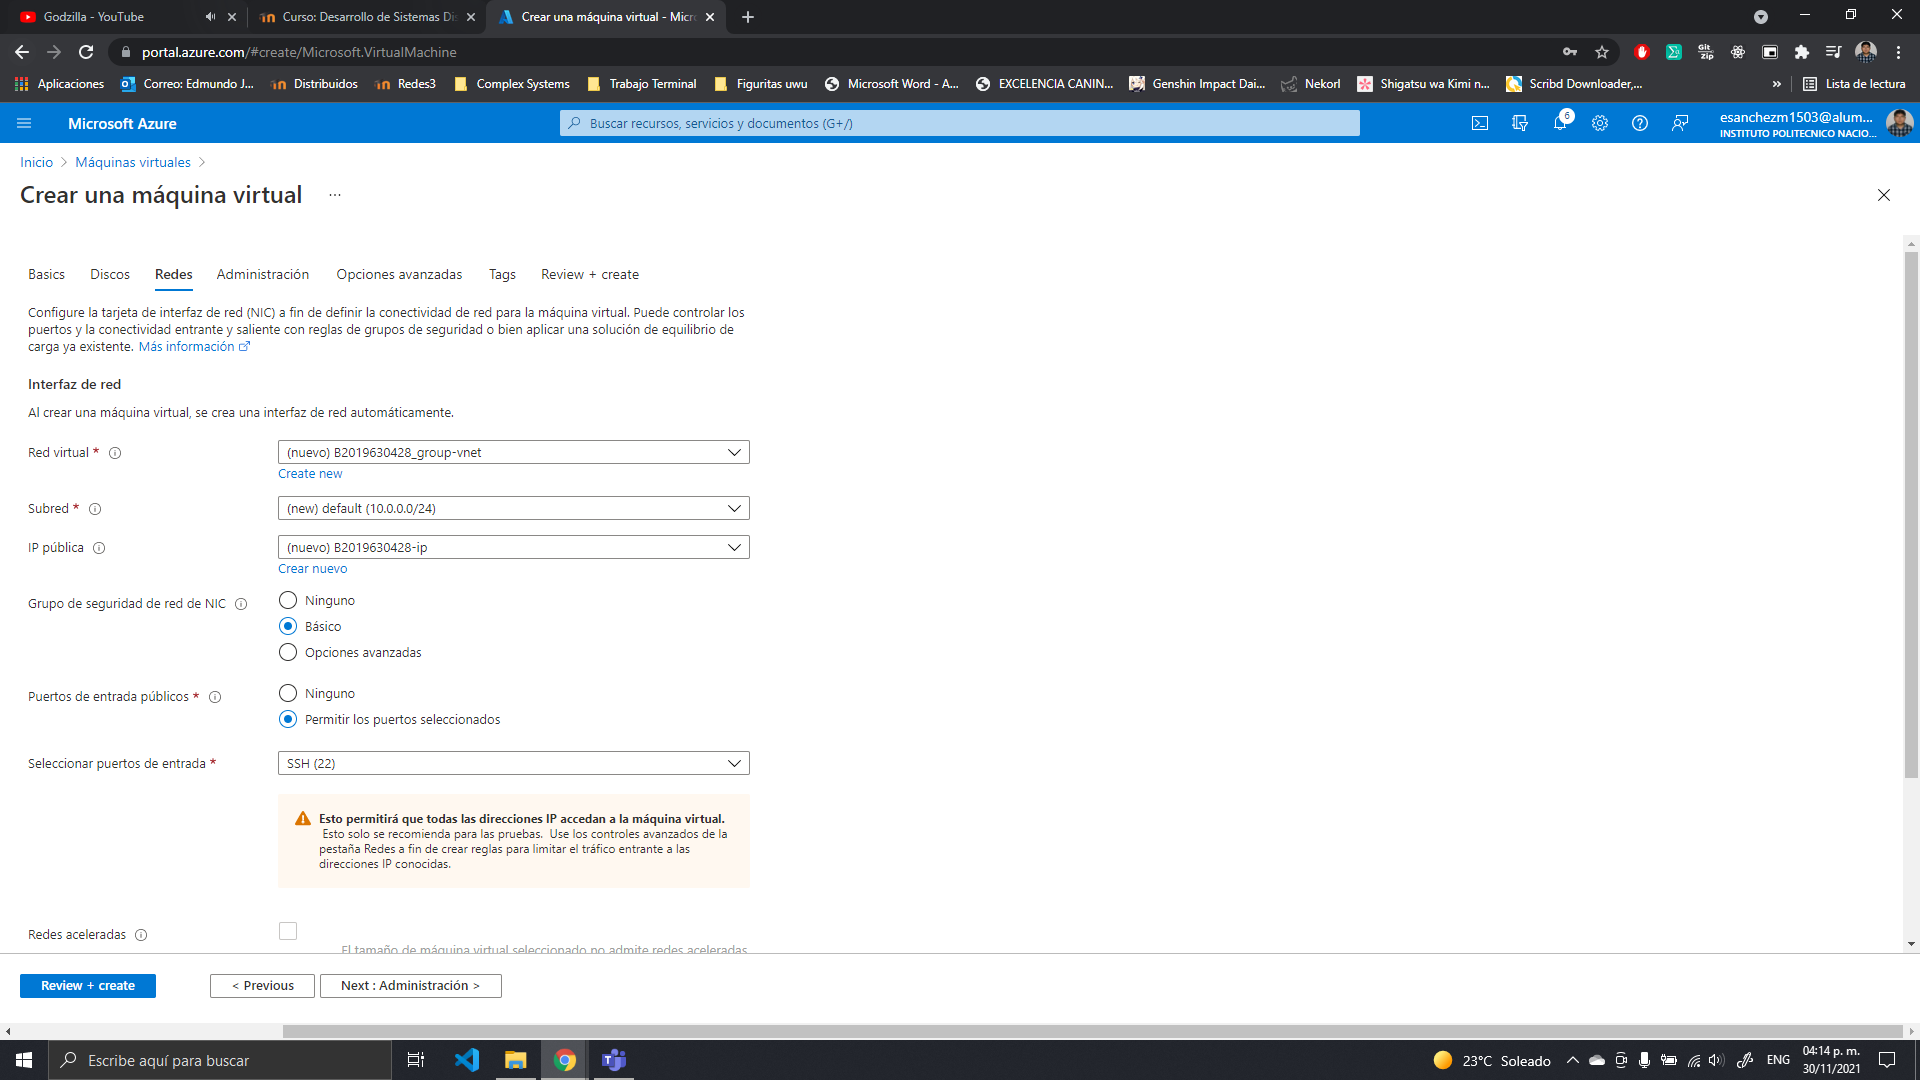
\includegraphics[scale=0.34]{resources/datosredes.png}
			\caption{Información sobre la redes. }\label{fig:picture}
		\end{figure}
		\begin{figure}[H]
			\centering
			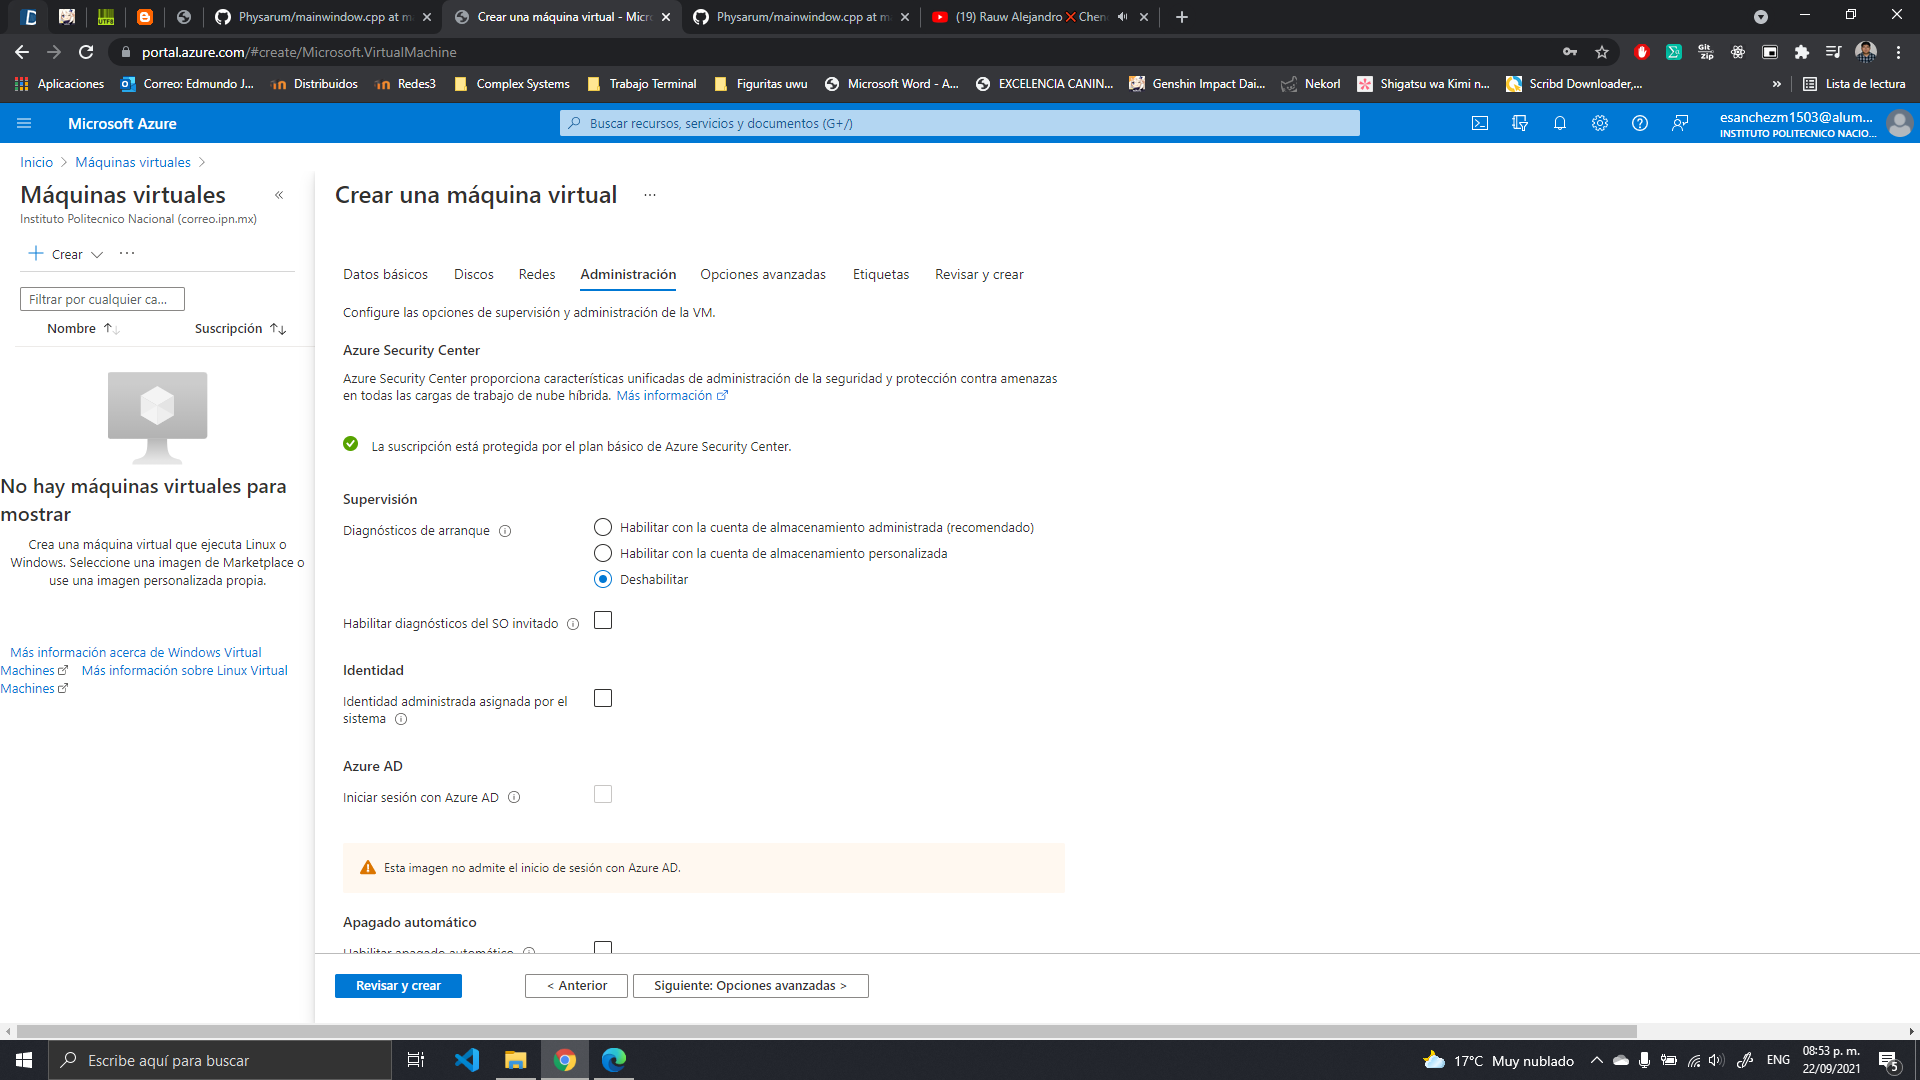
\includegraphics[scale=0.34]{resources/datosadministracion.png}
			\caption{Configuración de la administración. }\label{fig:picture}
		\end{figure}
		\begin{figure}[H]
			\centering
			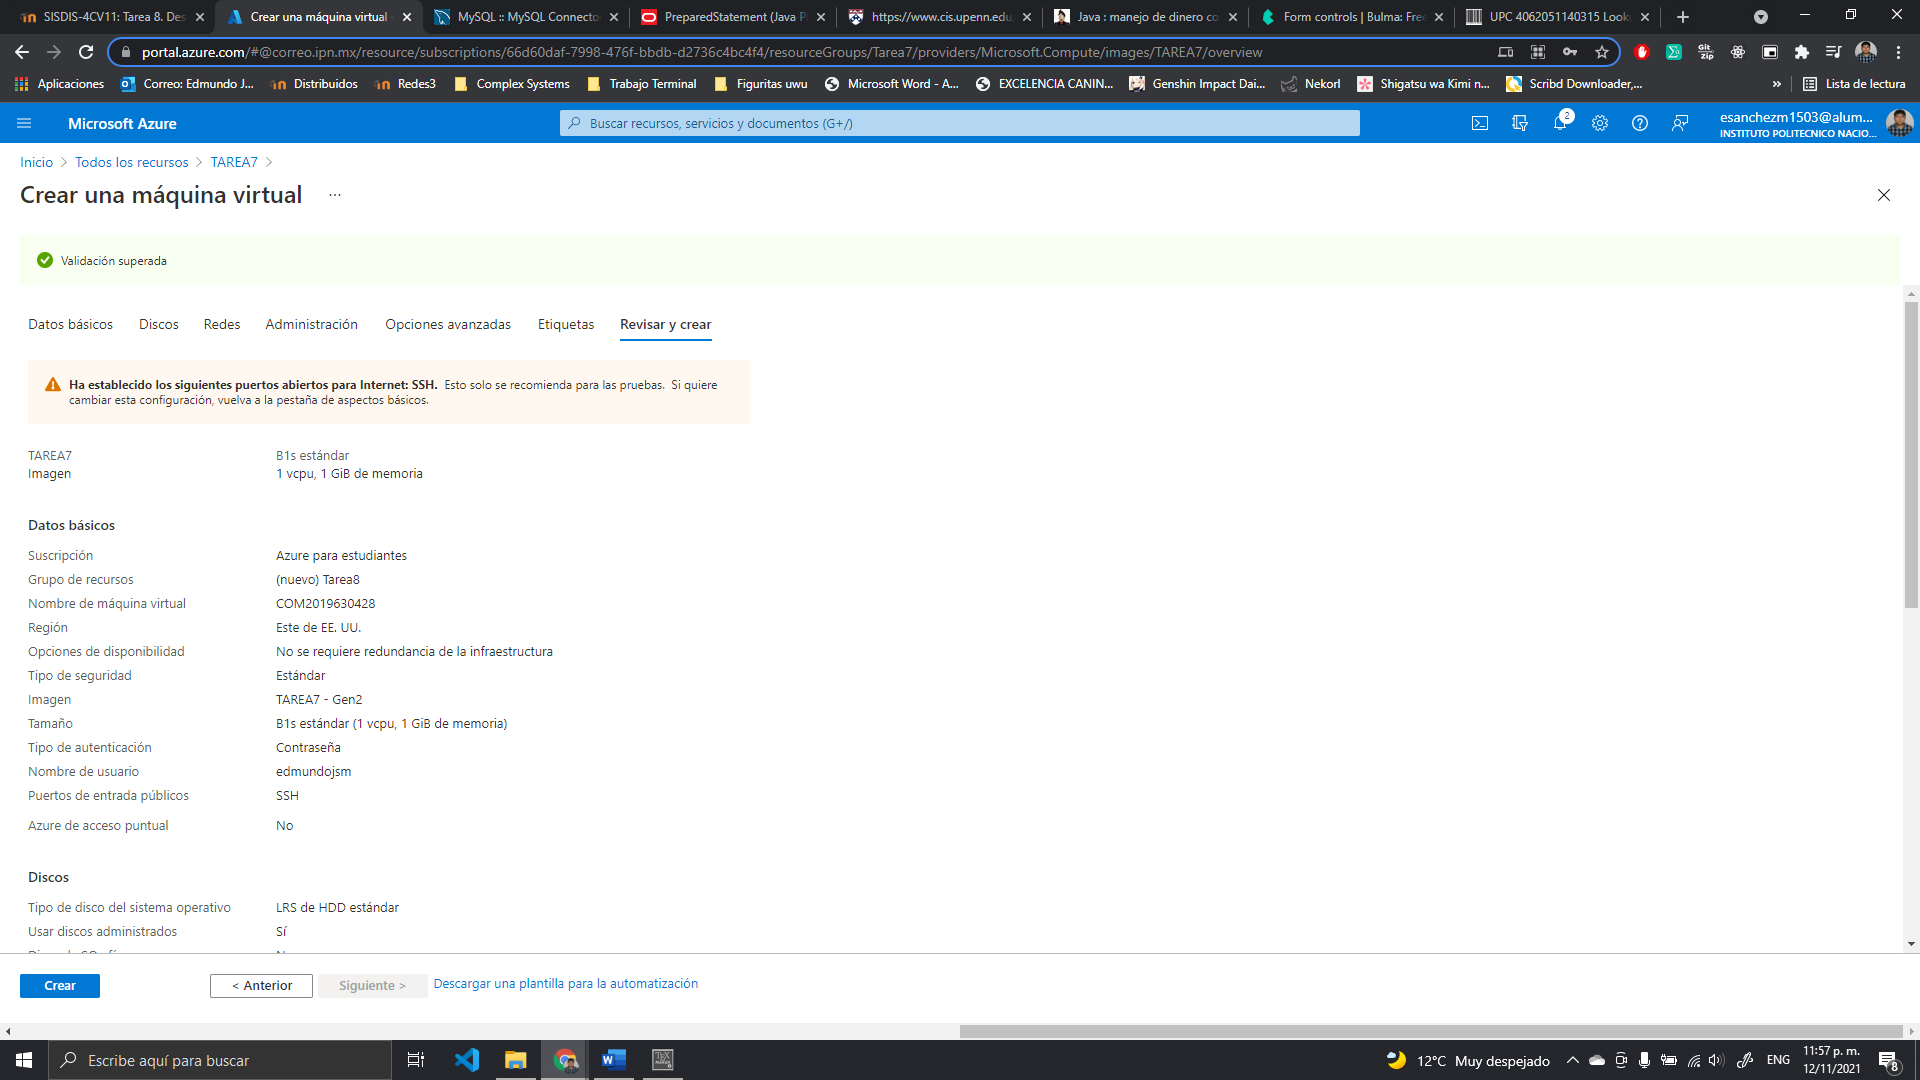
\includegraphics[scale=0.34]{resources/revisarycrear.png}
			\caption{Creación de la maquina virtual. }\label{fig:picture}
		\end{figure}
		\begin{figure}[H]
			\centering
			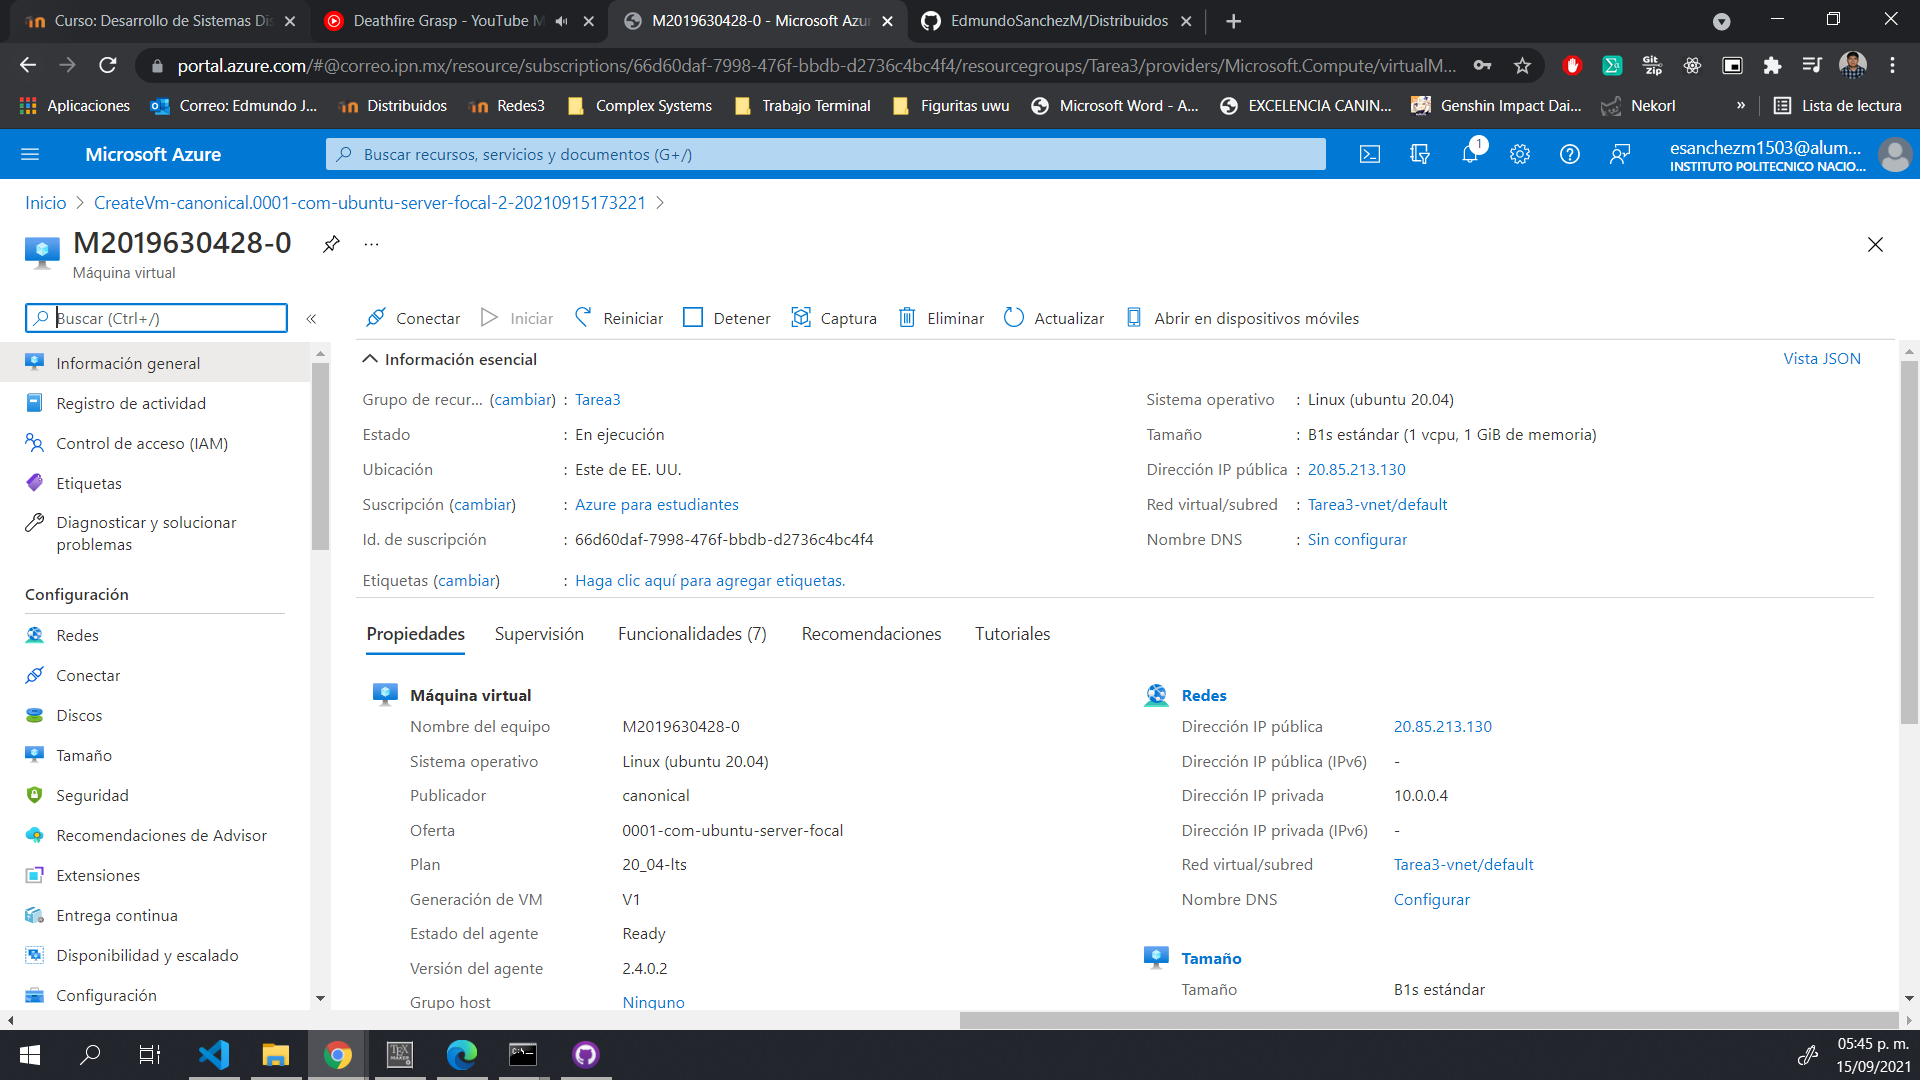
\includegraphics[scale=0.34]{resources/Panelcontrol.png}
			\caption{Panel de control de la maquina virtual. }\label{fig:picture}
		\end{figure}
Una vez creada la máquina virtual se procedió ir al apartado se accedido al apartado de conectar para poder descargar nuestro archivo RPD que es necesario para hacer la conexión con nuestra máquina virtual, esto se puede ver en la imagen 9.
		\begin{figure}[H]
			\centering
			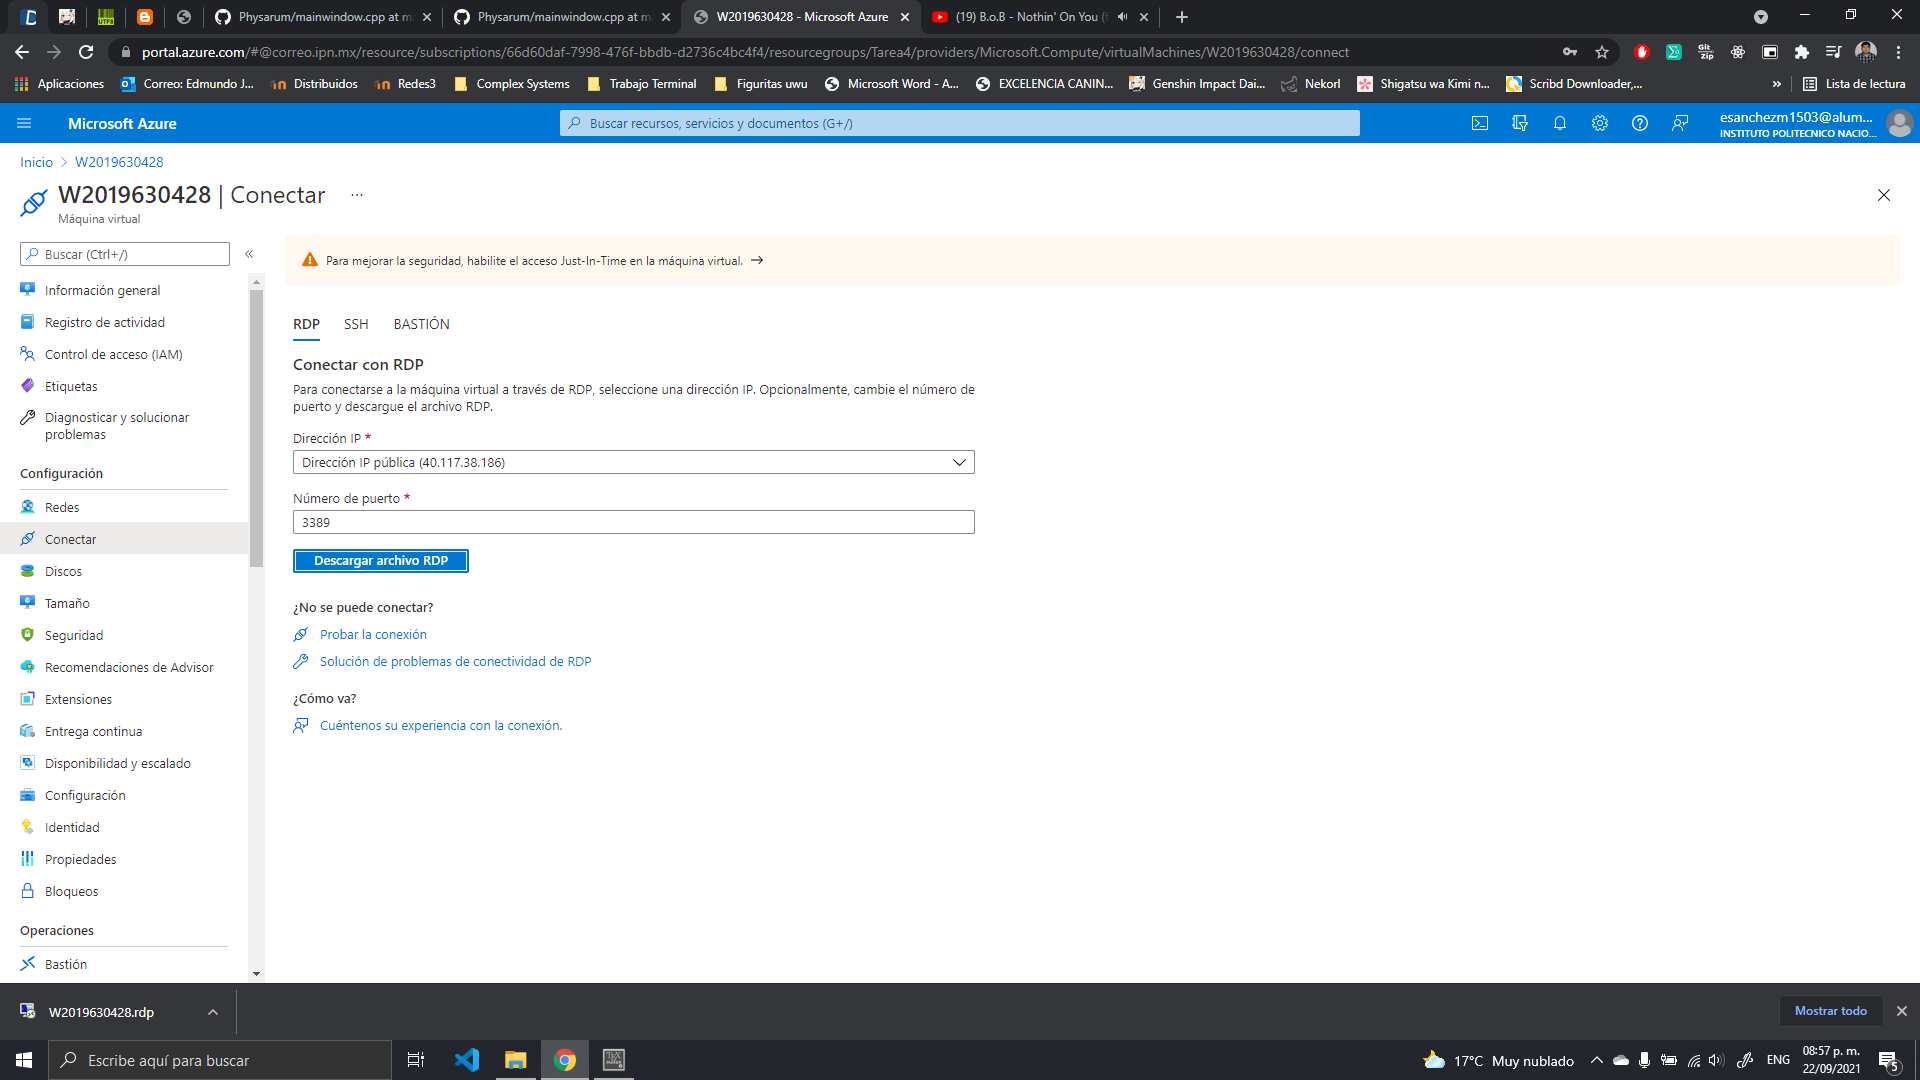
\includegraphics[scale=0.34]{resources/descargarpd.png}
			\caption{Descarga del archivo RPD. }\label{fig:picture}
		\end{figure}
Mientras se realizaba la descarga del archivo RPD, se procedió a crear un disco lógico local en la unidad F, como dato adicional, la figura 10 tiene diferente fecha ya que el desarrollo de la practica empezó en el inicio de la semana de entrega.
		\begin{figure}[H]
			\centering
			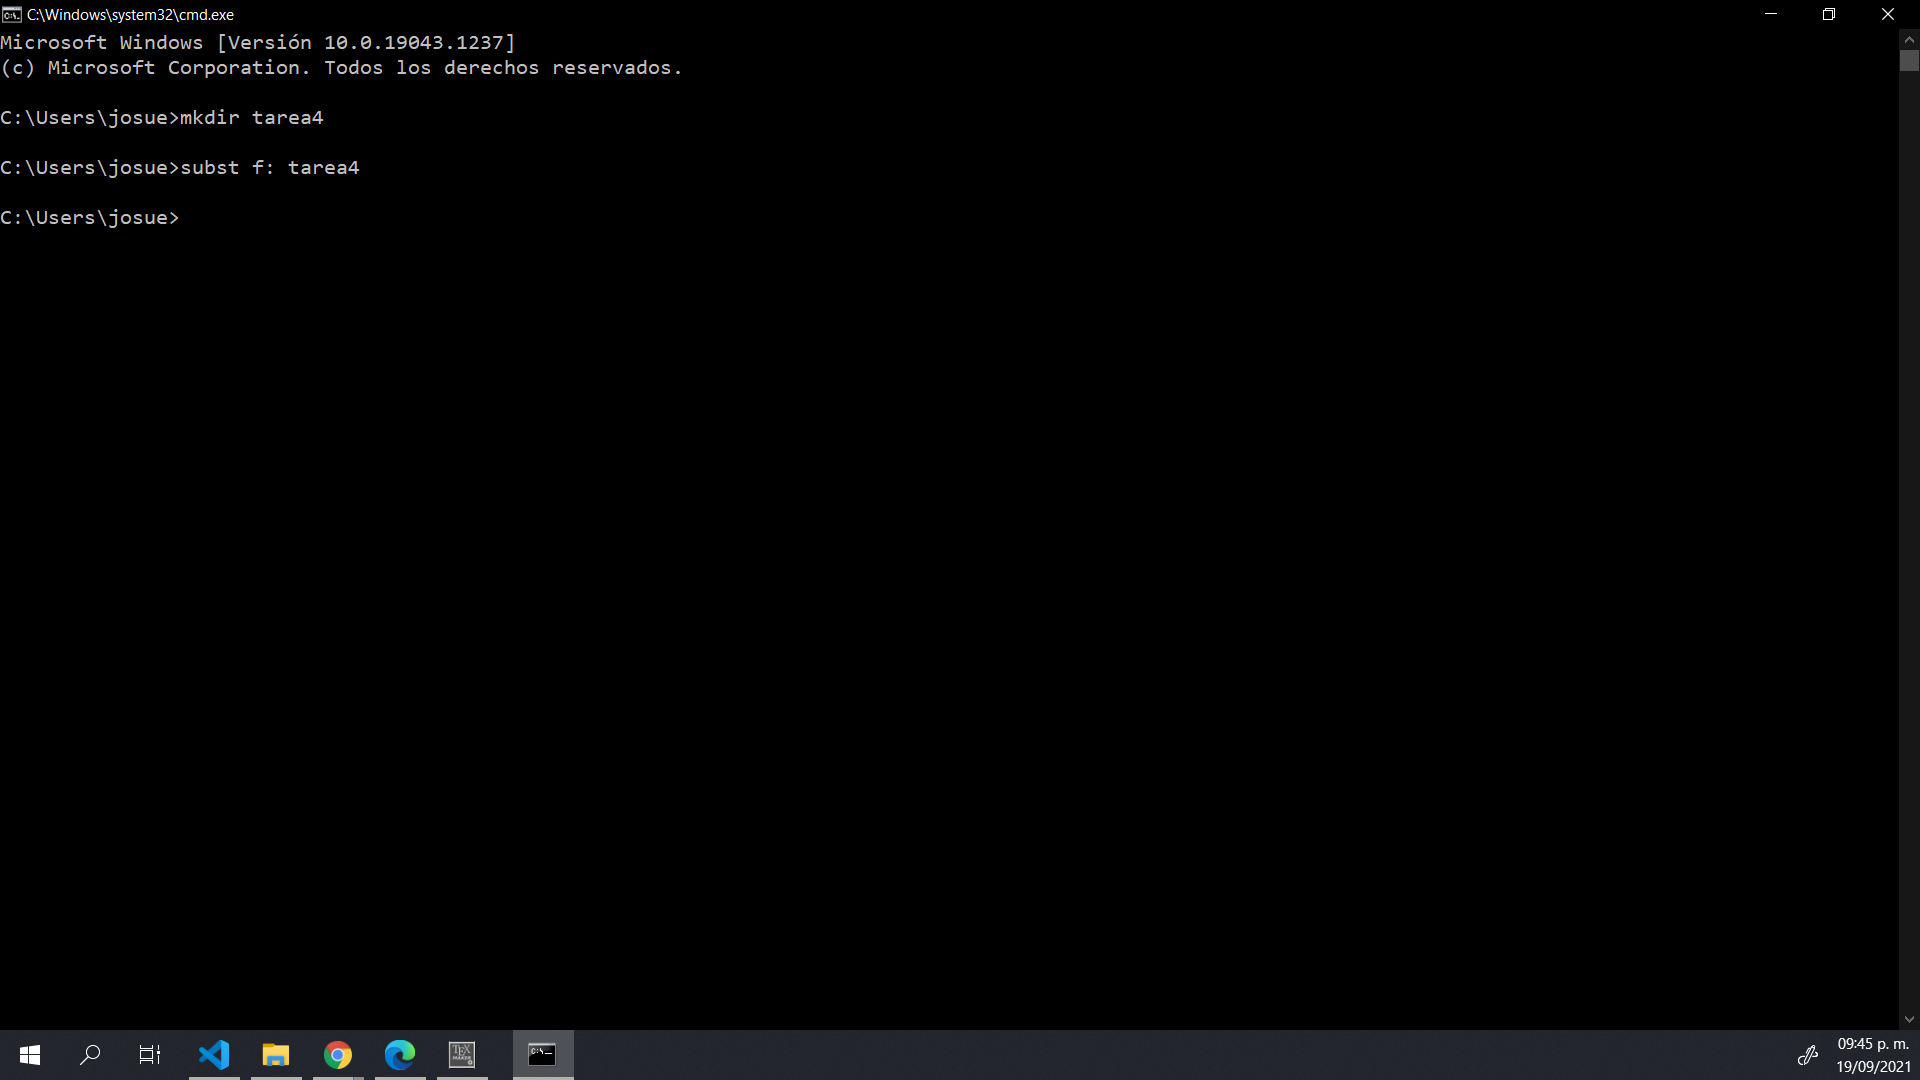
\includegraphics[scale=0.34]{resources/discologico.png}
			\caption{Creación de disco lógico. }\label{fig:picture}
		\end{figure}
Al tener todo listo se procede a editar nuestro archivo RPD para compartir recursos, se compartirá el disco lógico recientemente creado, una vez editado se procede a realizar la conexión con nuestra maquina virtual, todo lo anterior se puede ver de la figura 11 a la 13. Mientras se realizaba lo anterior decidí aprovechar el tiempo y descargar el JDK 8u202 para poder instalarlo en la maquina virtual como se ve en la figura 14, una vez terminada la descarga copie el JDK así como el archivo Chat.java en nuestro disco lógico (figura 15).
		\begin{figure}[H]
			\centering
			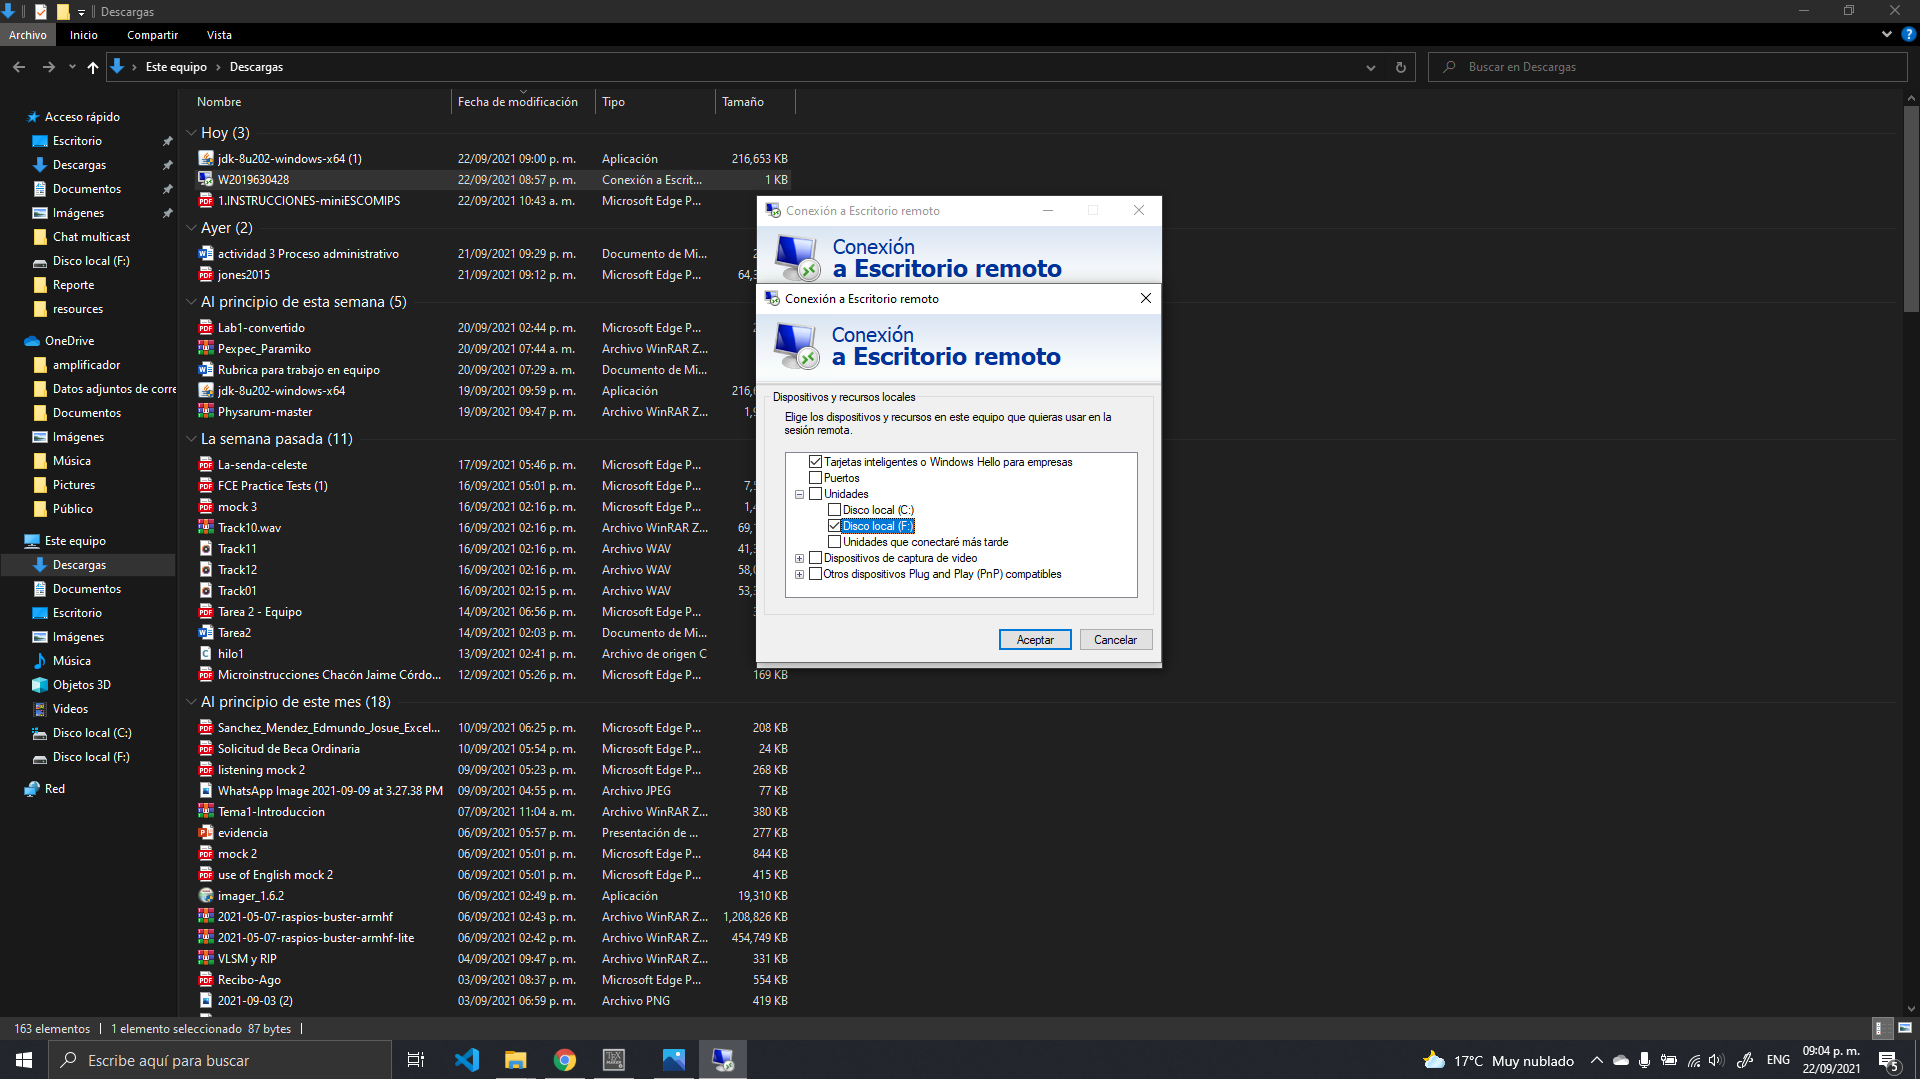
\includegraphics[scale=0.34]{resources/recursoscompartidos.png}
			\caption{Editando archivo RPD para compartir nuestro disco lógico.}\label{fig:picture}
		\end{figure}
		\begin{figure}[H]
			\centering
			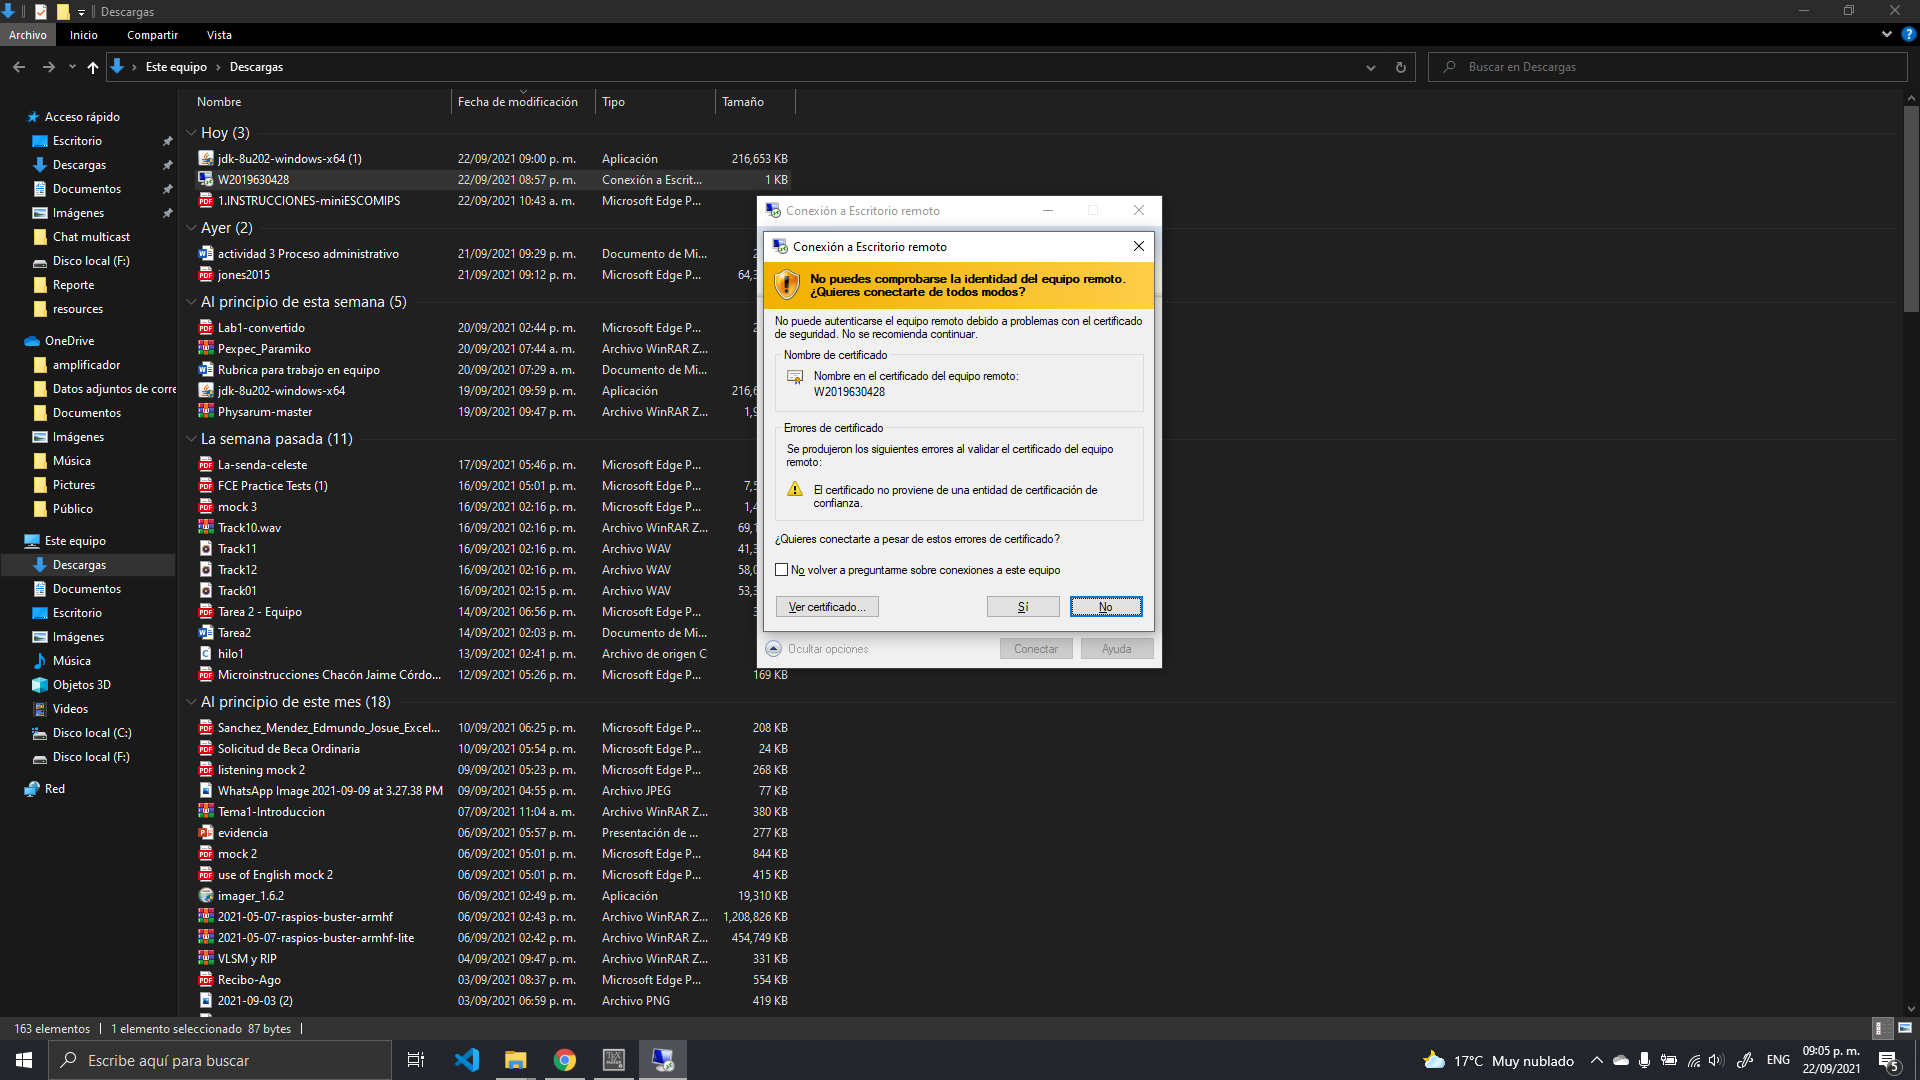
\includegraphics[scale=0.34]{resources/inicioconexion.png}
			\caption{Inicio de conexión con la maquina virtual.}\label{fig:picture}
		\end{figure}
		\begin{figure}[H]
			\centering
			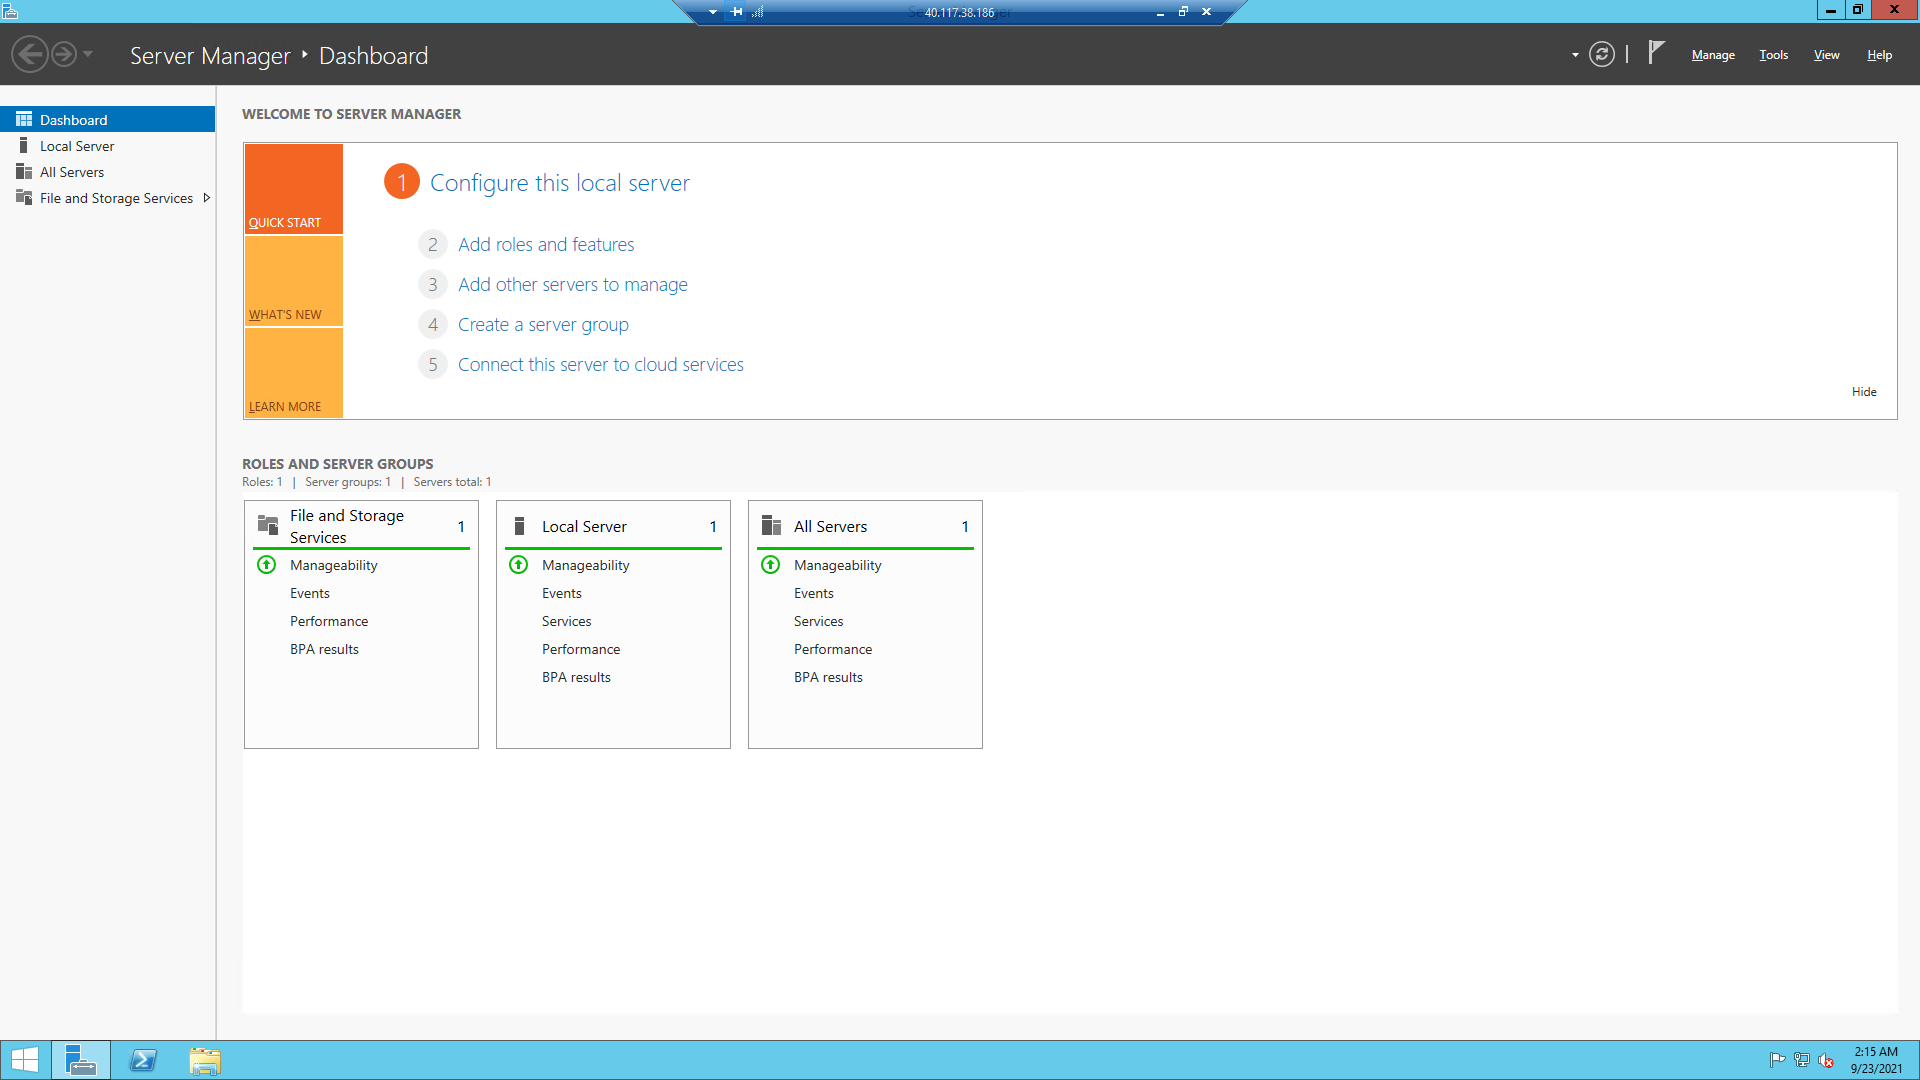
\includegraphics[scale=0.34]{resources/conexionok.png}
			\caption{Conexión realizada de manera exitosa con la maquina virtual.}\label{fig:picture}
		\end{figure}
		\begin{figure}[H]
			\centering
			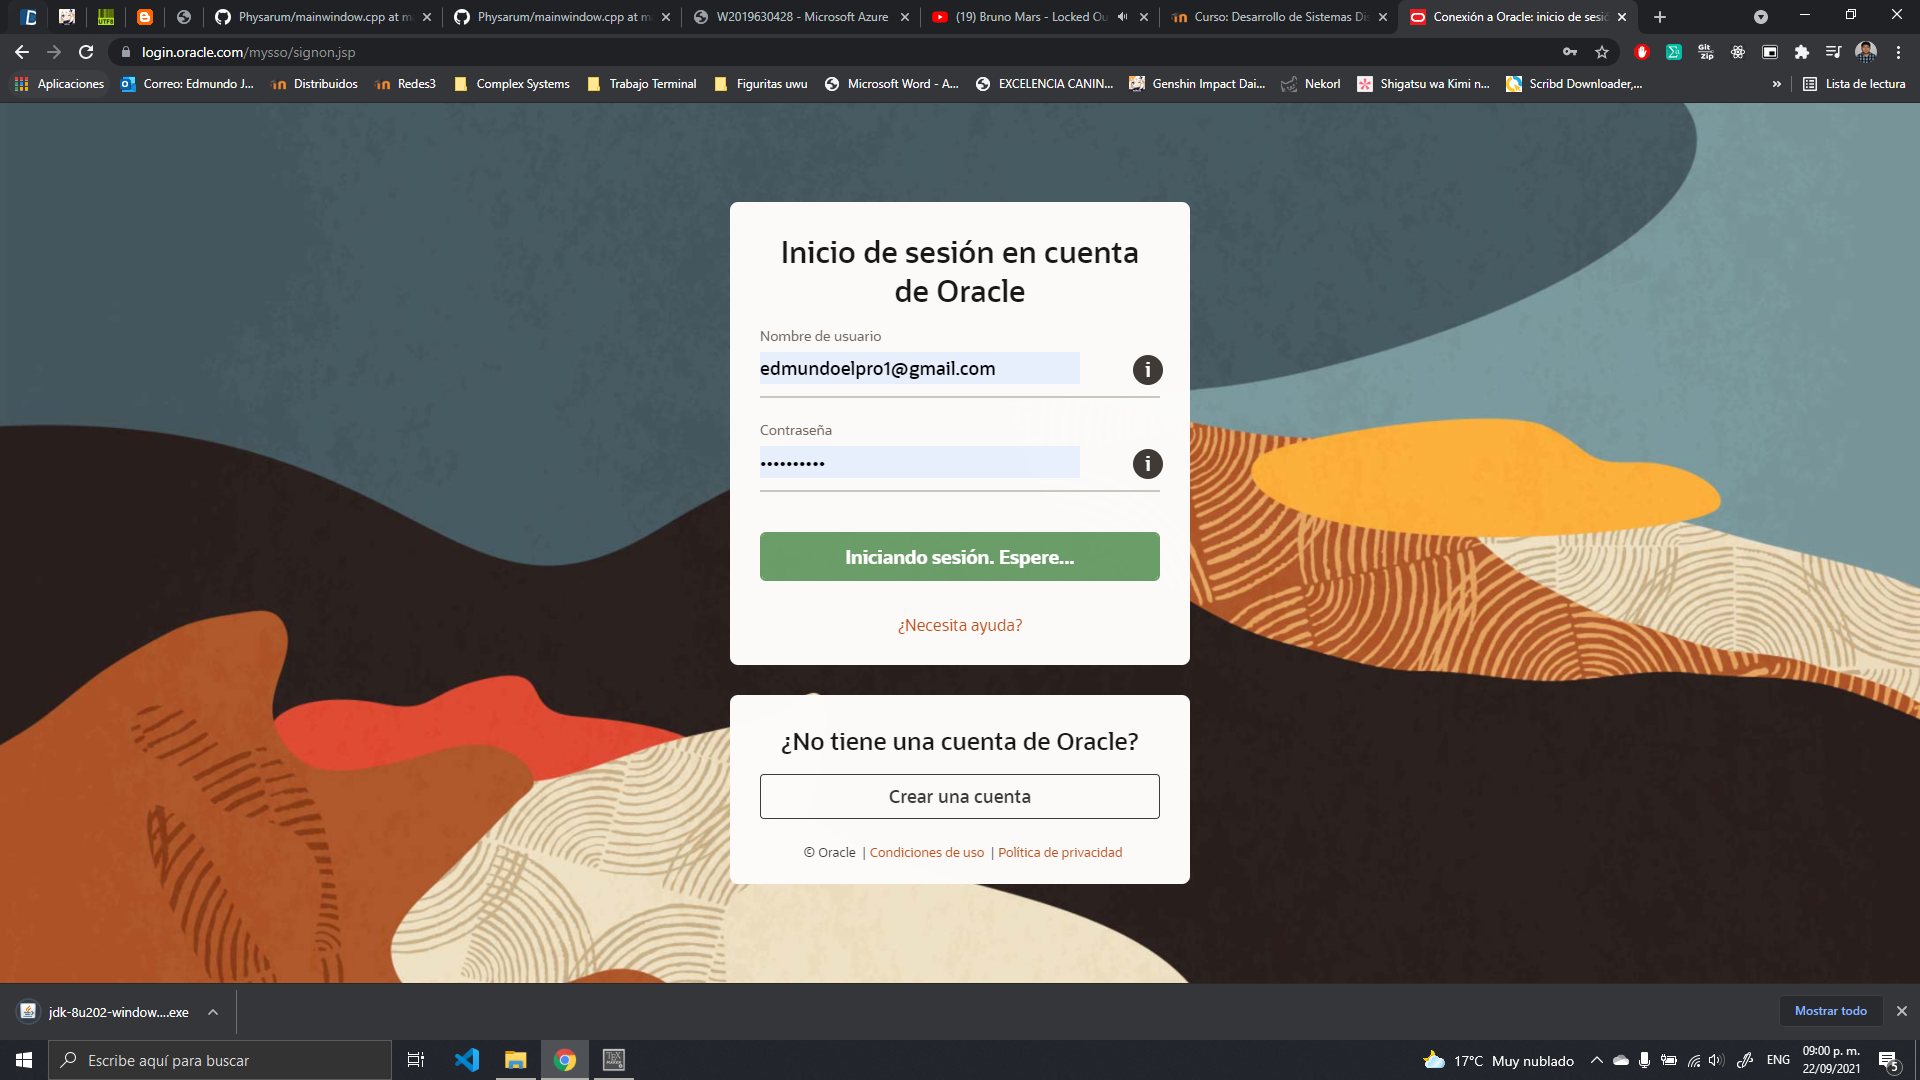
\includegraphics[scale=0.34]{resources/descargajdk.png}
			\caption{Descarga del JDK 8u202.}\label{fig:picture}
		\end{figure}
		\begin{figure}[H]
			\centering
			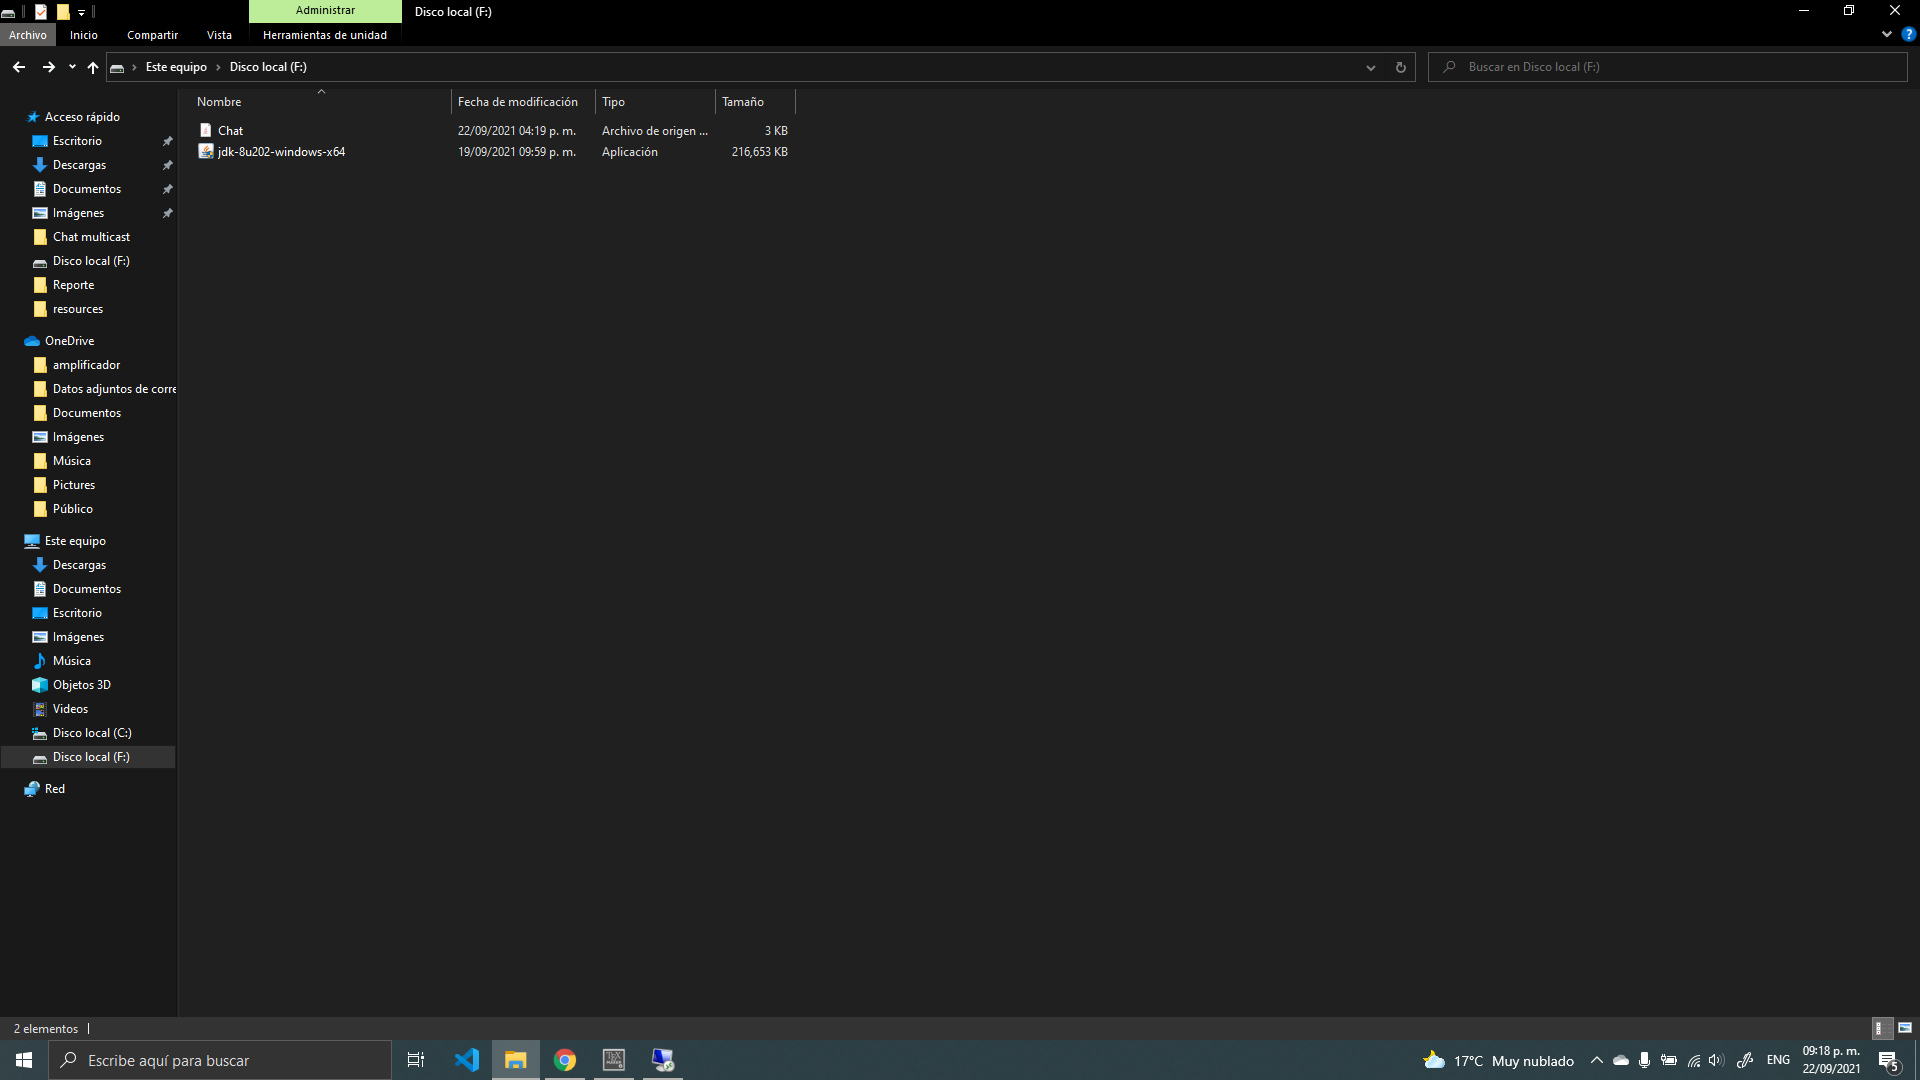
\includegraphics[scale=0.34]{resources/contenidoscarpetalocal.png}
			\caption{Contenido del disco lógico.}\label{fig:picture}
		\end{figure}
Me gustaría comentar que no me fue posible tomar la screenshot en donde saliera tanto la máquina virtual como mi barra de tareas, ya que no se me permitía cambiar la resolución de la máquina y cuando lo hacía de manera manual no se visualizaba por completo la máquina virtual.
Una vez hecho todo lo anterior solo nos queda instalar Java, agregar JAVA\_ HOME como variable de sistema, agregarla a path, reiniciar, ademas de añadir el distribución del teclado latinoamericano para realizar las pruebas y eso seria todo. Esto se puede ver desde la figura 16 a la 20.
		\begin{figure}[H]
			\centering
			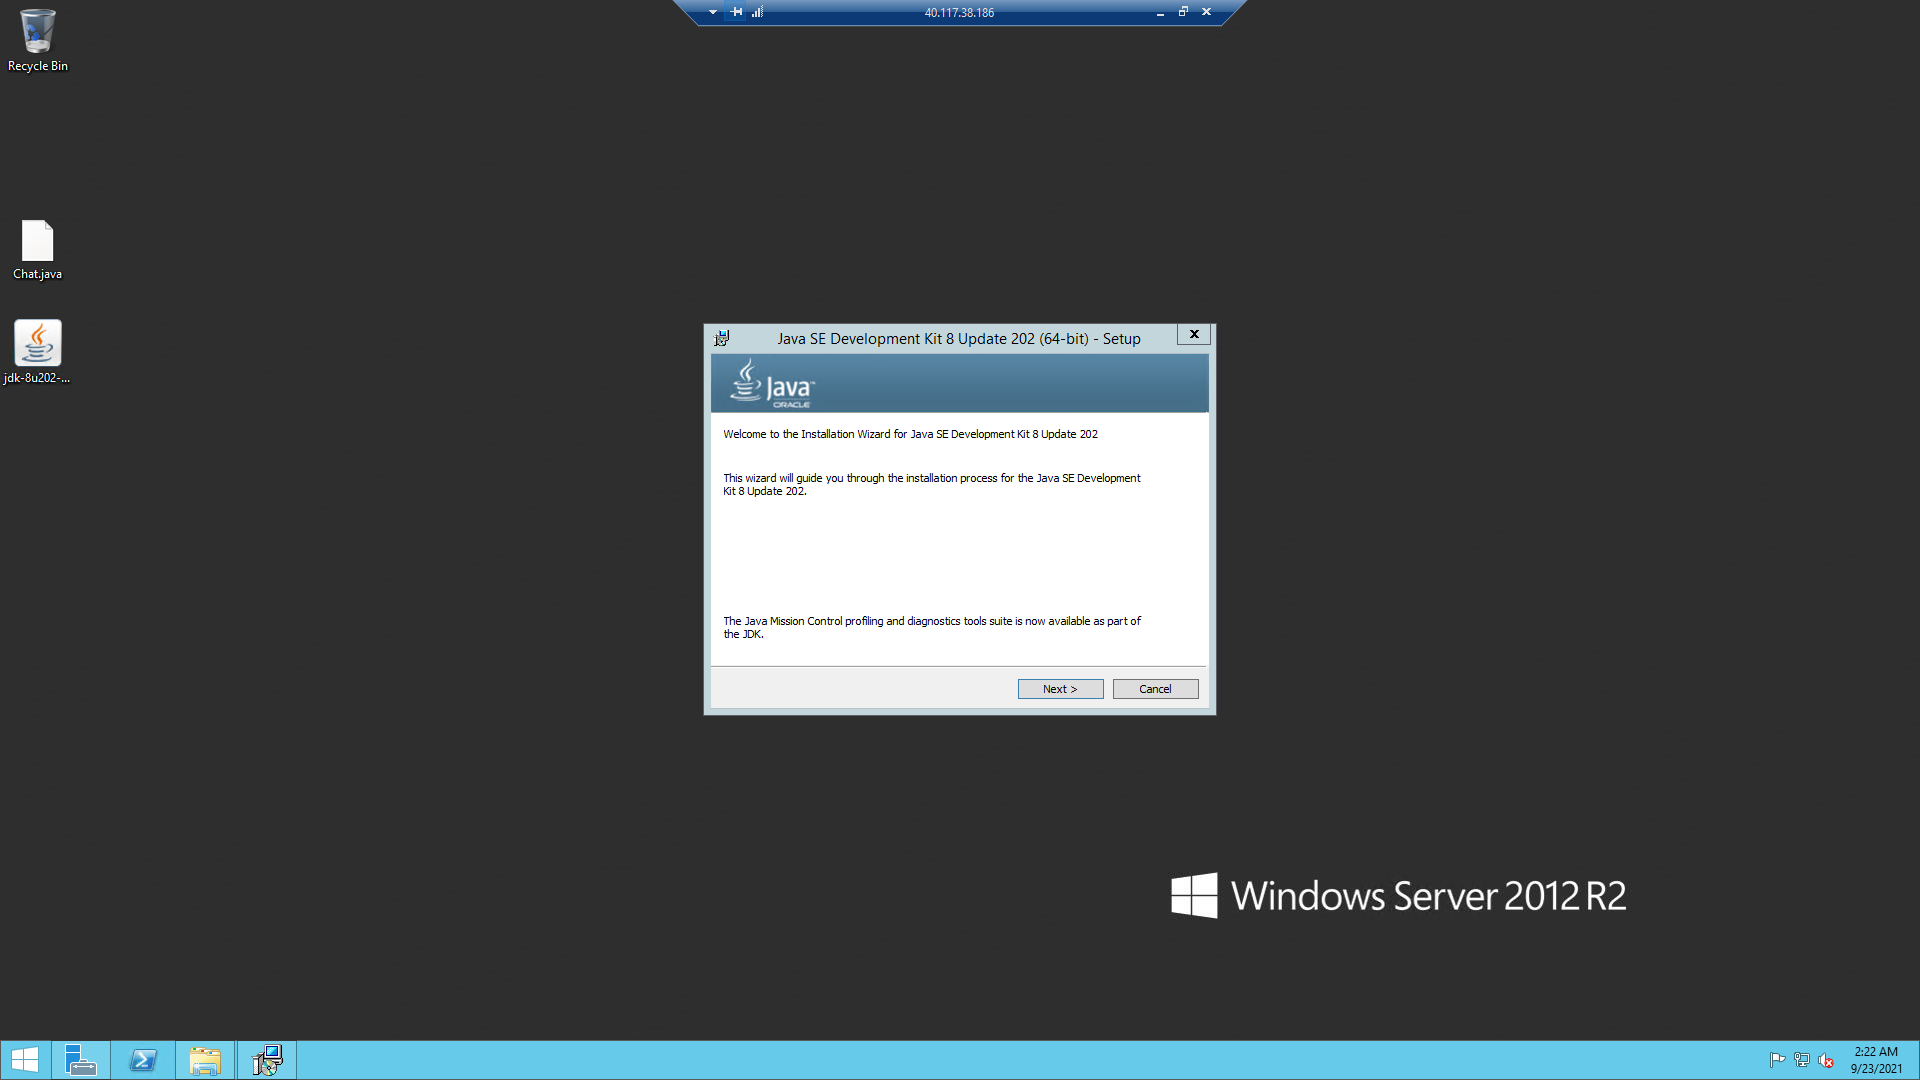
\includegraphics[scale=0.34]{resources/inicioinstalacionjava.png}
			\caption{Iniciando instalación de Java.}\label{fig:picture}
		\end{figure}
		\begin{figure}[H]
			\centering
			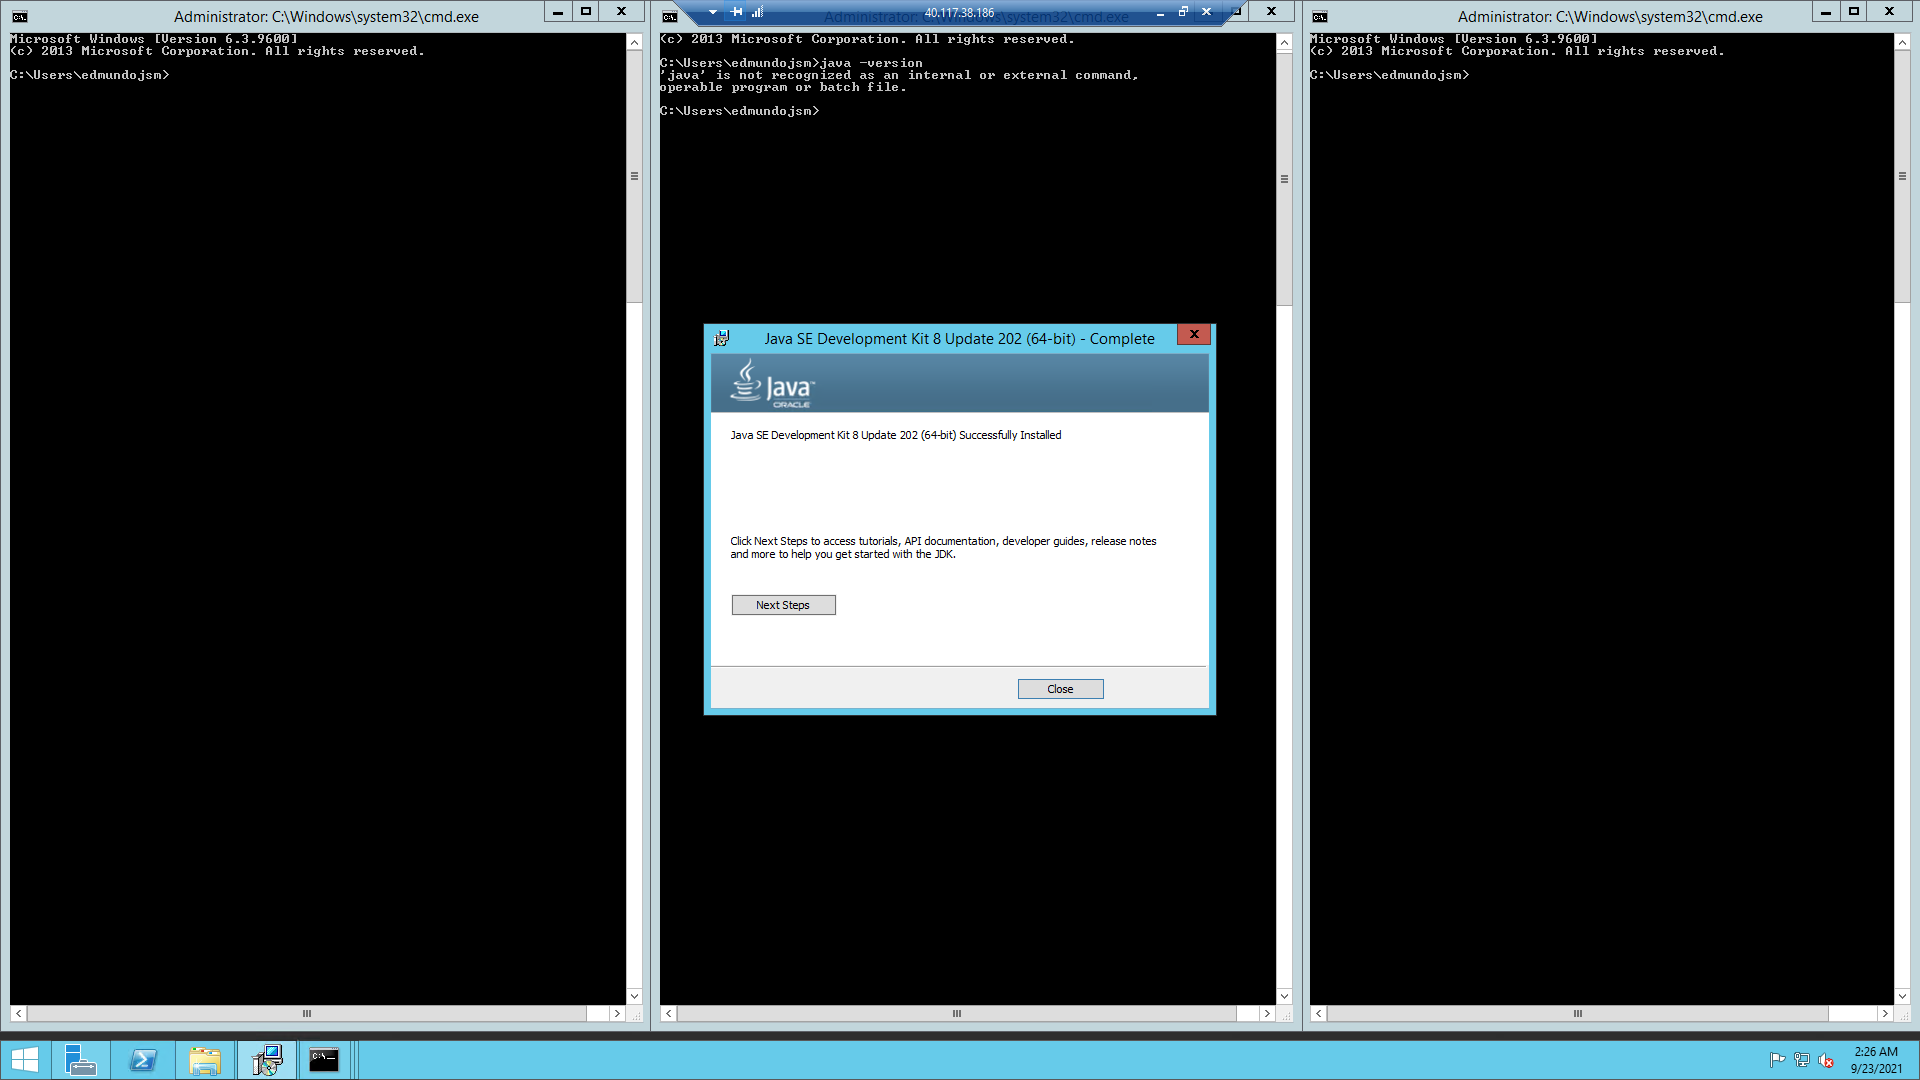
\includegraphics[scale=0.34]{resources/instalacionjavafinalizada.png}
			\caption{Fin de la instalación de Java.}\label{fig:picture}
		\end{figure}
		\begin{figure}[H]
			\centering
			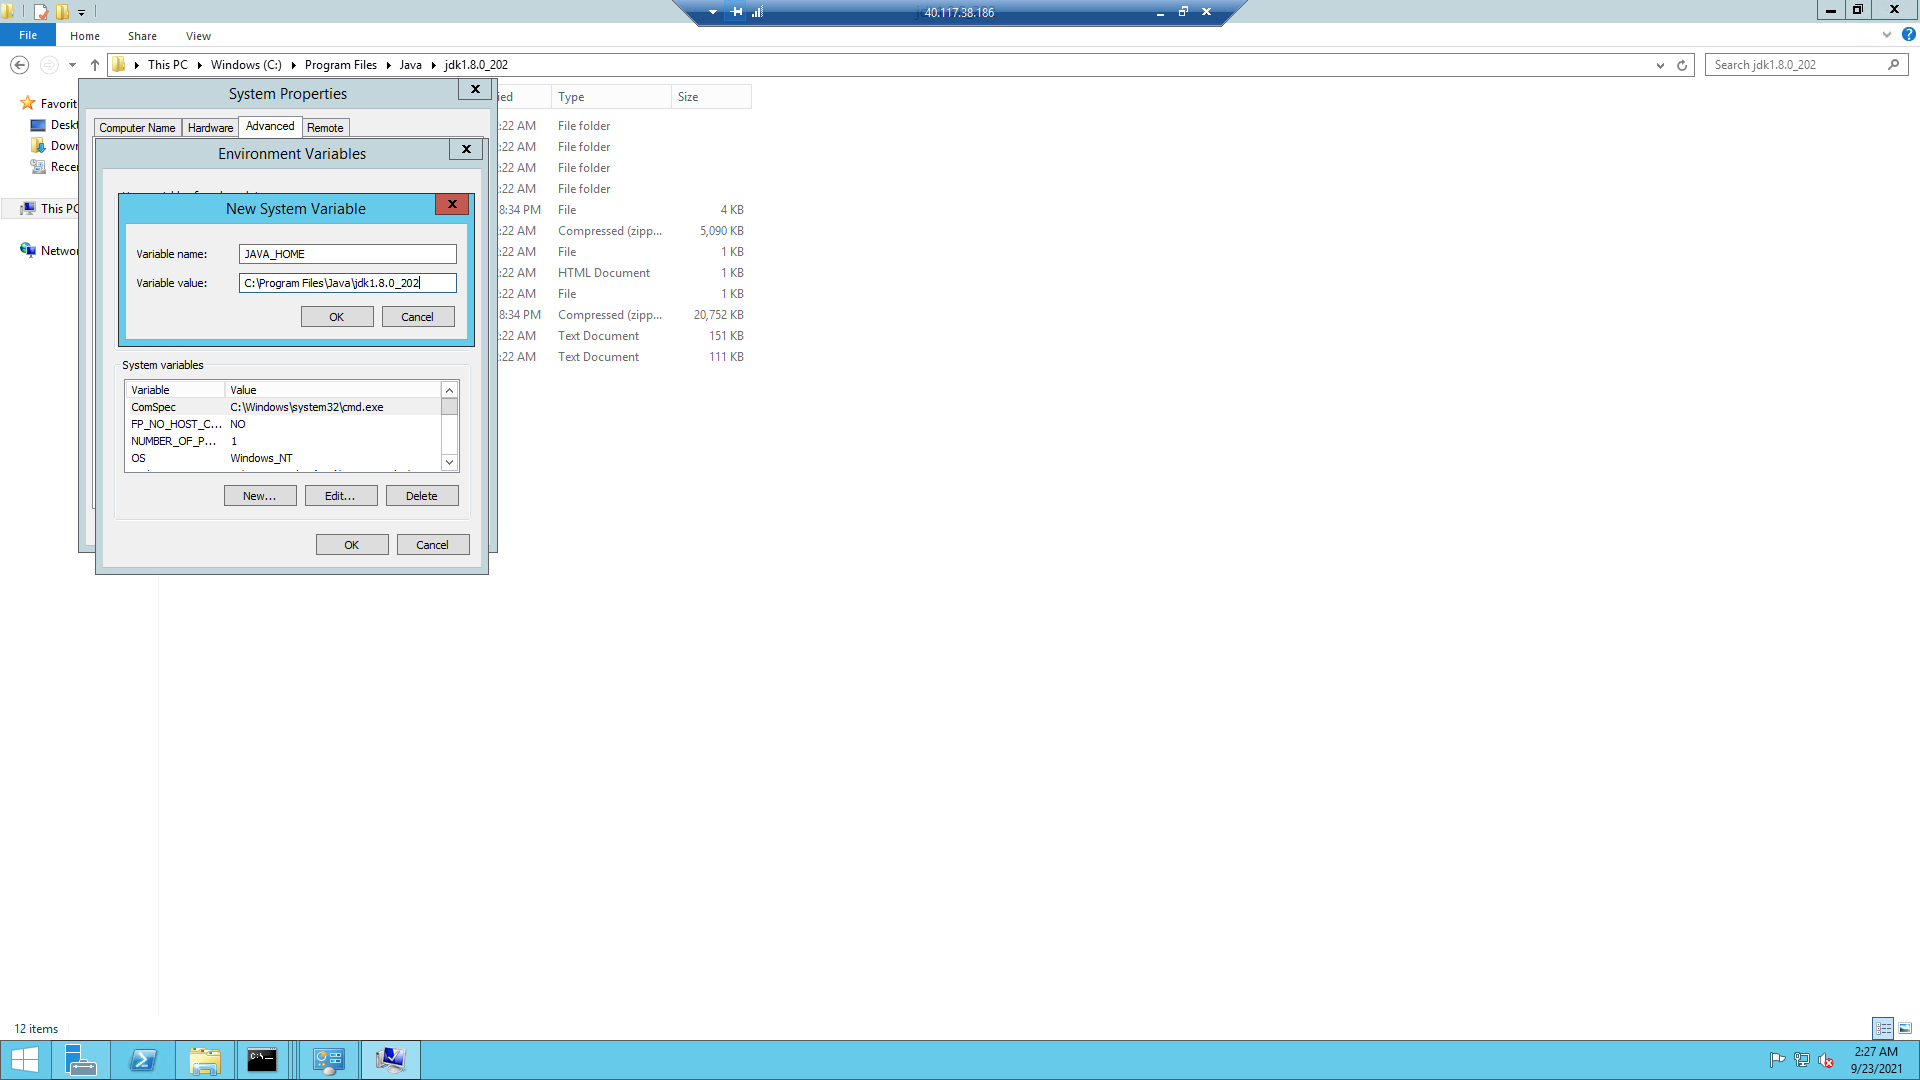
\includegraphics[scale=0.34]{resources/javahome.png}
			\caption{Añadiendo JAVA\_ HOME.}\label{fig:picture}
		\end{figure}
		\begin{figure}[H]
			\centering
			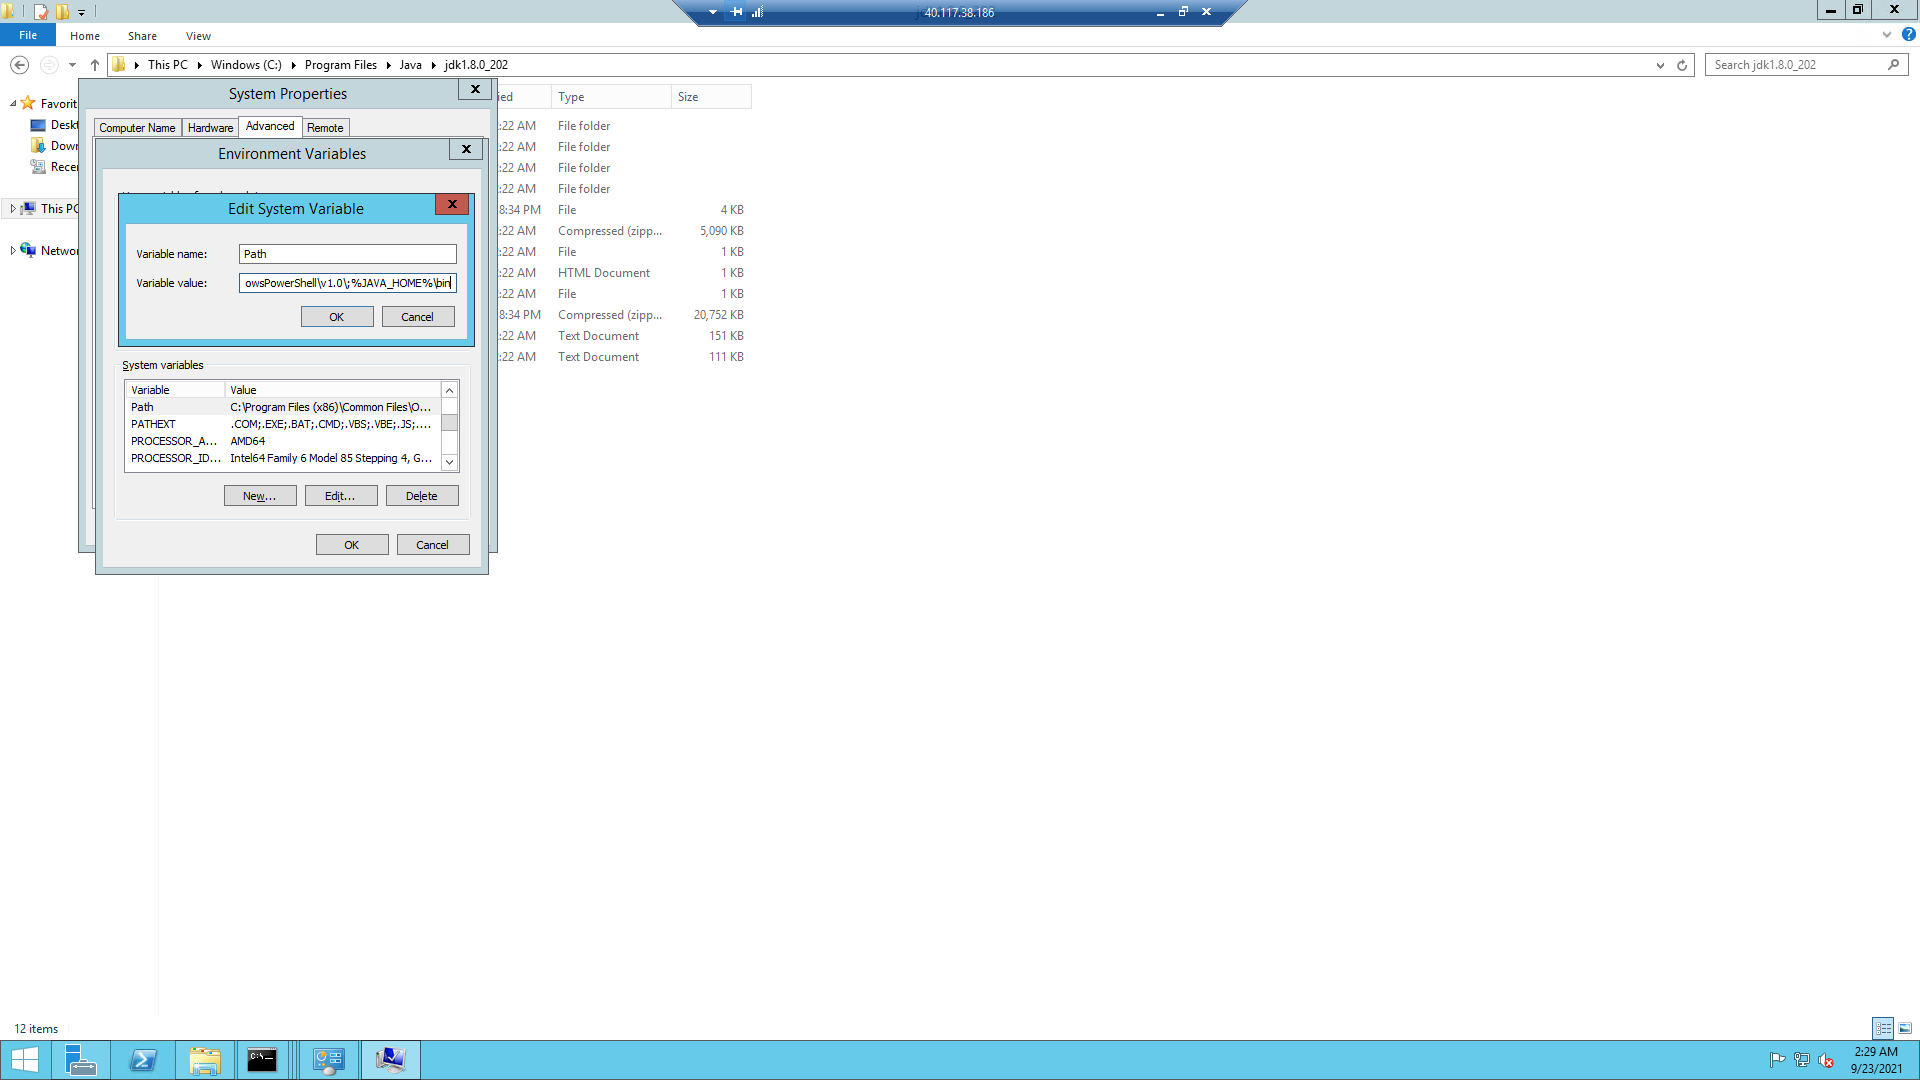
\includegraphics[scale=0.34]{resources/actualizapath.png}
			\caption{Actualizando variable path.}\label{fig:picture}
		\end{figure}
		\begin{figure}[H]
			\centering
			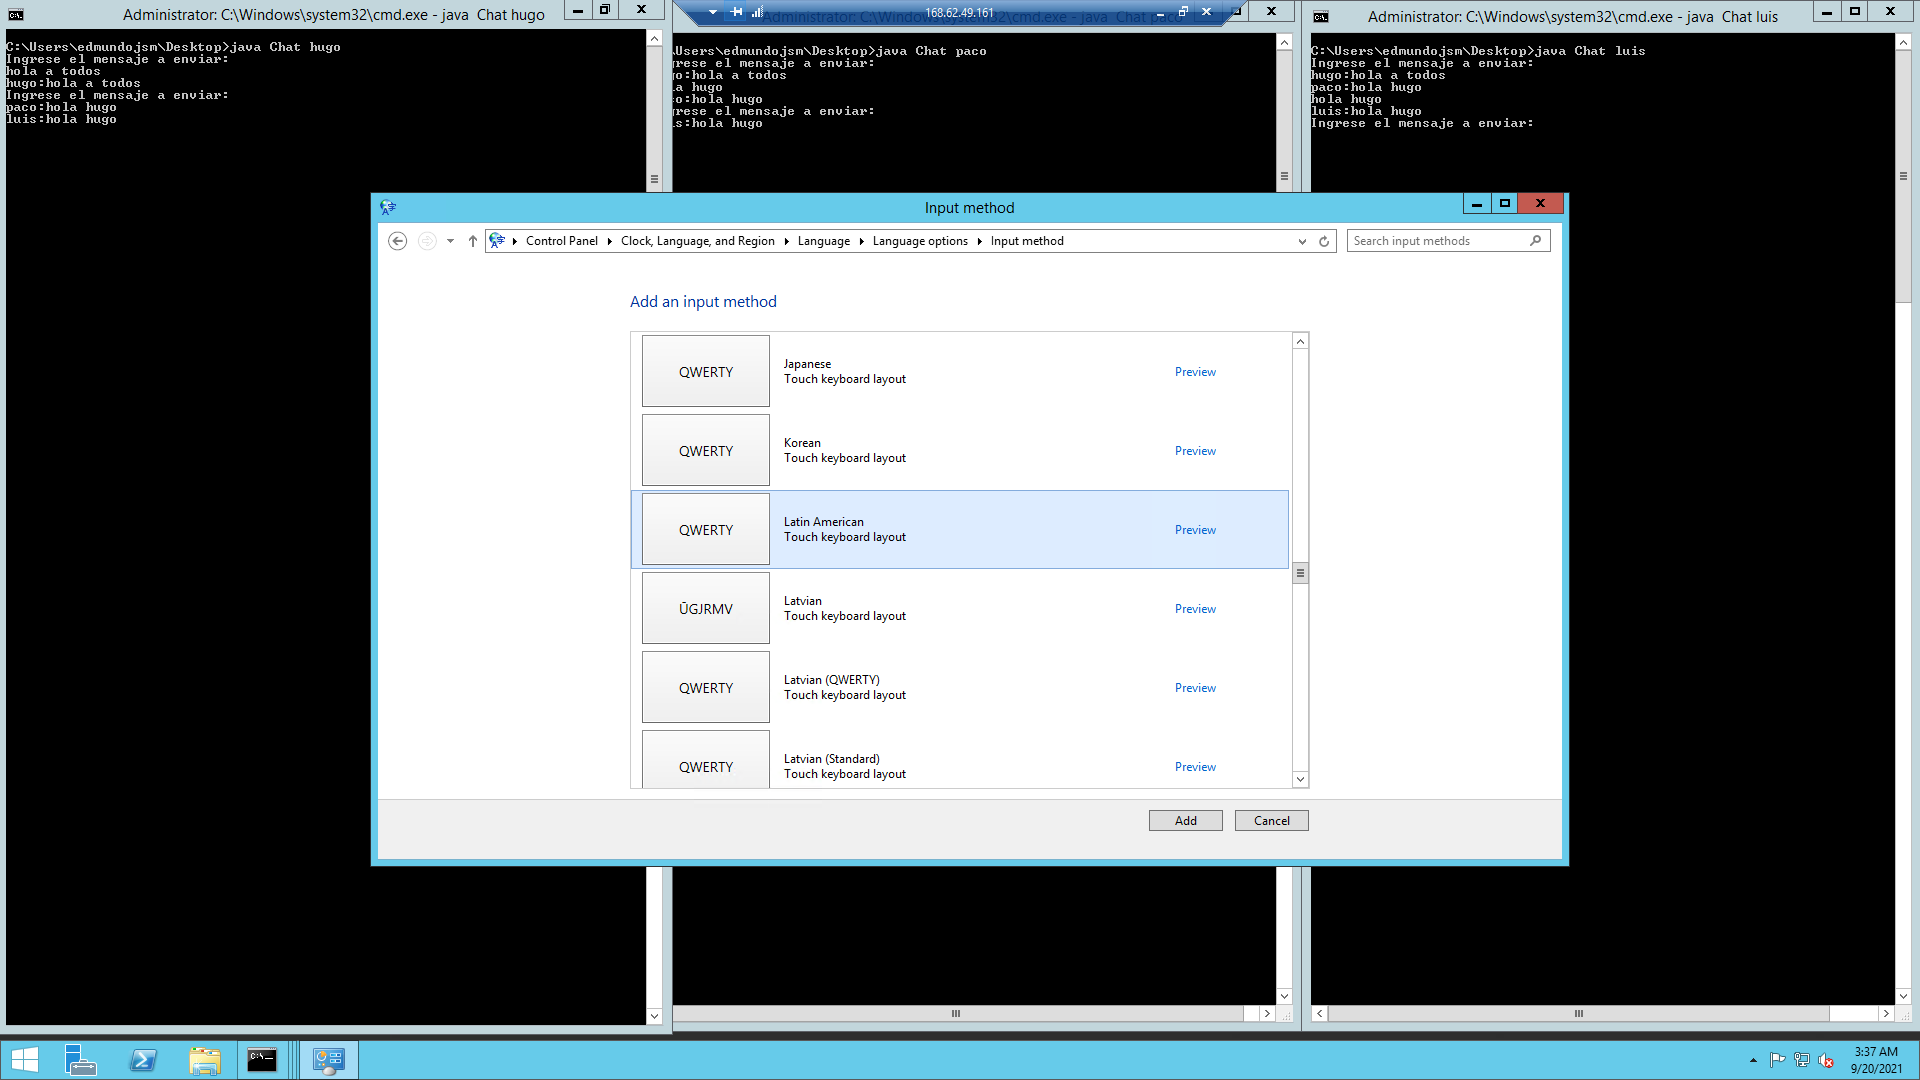
\includegraphics[scale=0.34]{resources/cambiarditribucionteclado.png}
			\caption{Agregando distribución de teclado.}\label{fig:picture}
		\end{figure}
		
		\subsection{Compilación del código}
		Al inicio del reporte comente que inicialmente use el código de pagina 1252 y UTF-8 para la practica pero esto no funciono, de hecho como podemos ver en la figura 21 vemos unos errores en el CMD de codificación incorrecta, por otro lado tenemos el PowerShell que si bien la codificación de entrada era correcta el desplegado no, al investigar resulta ser que esos cuadros salen ya que la codificación del carácter no se encuentra definida en la pagina de código, esto se puede ver si usamos el archivo Chatv1.java claramente este nombre tendra que cambiar a Chat ya que el nombre de la clase debe de ser el mismo que el nombre del archivo.
		\begin{figure}[H]
			\centering
			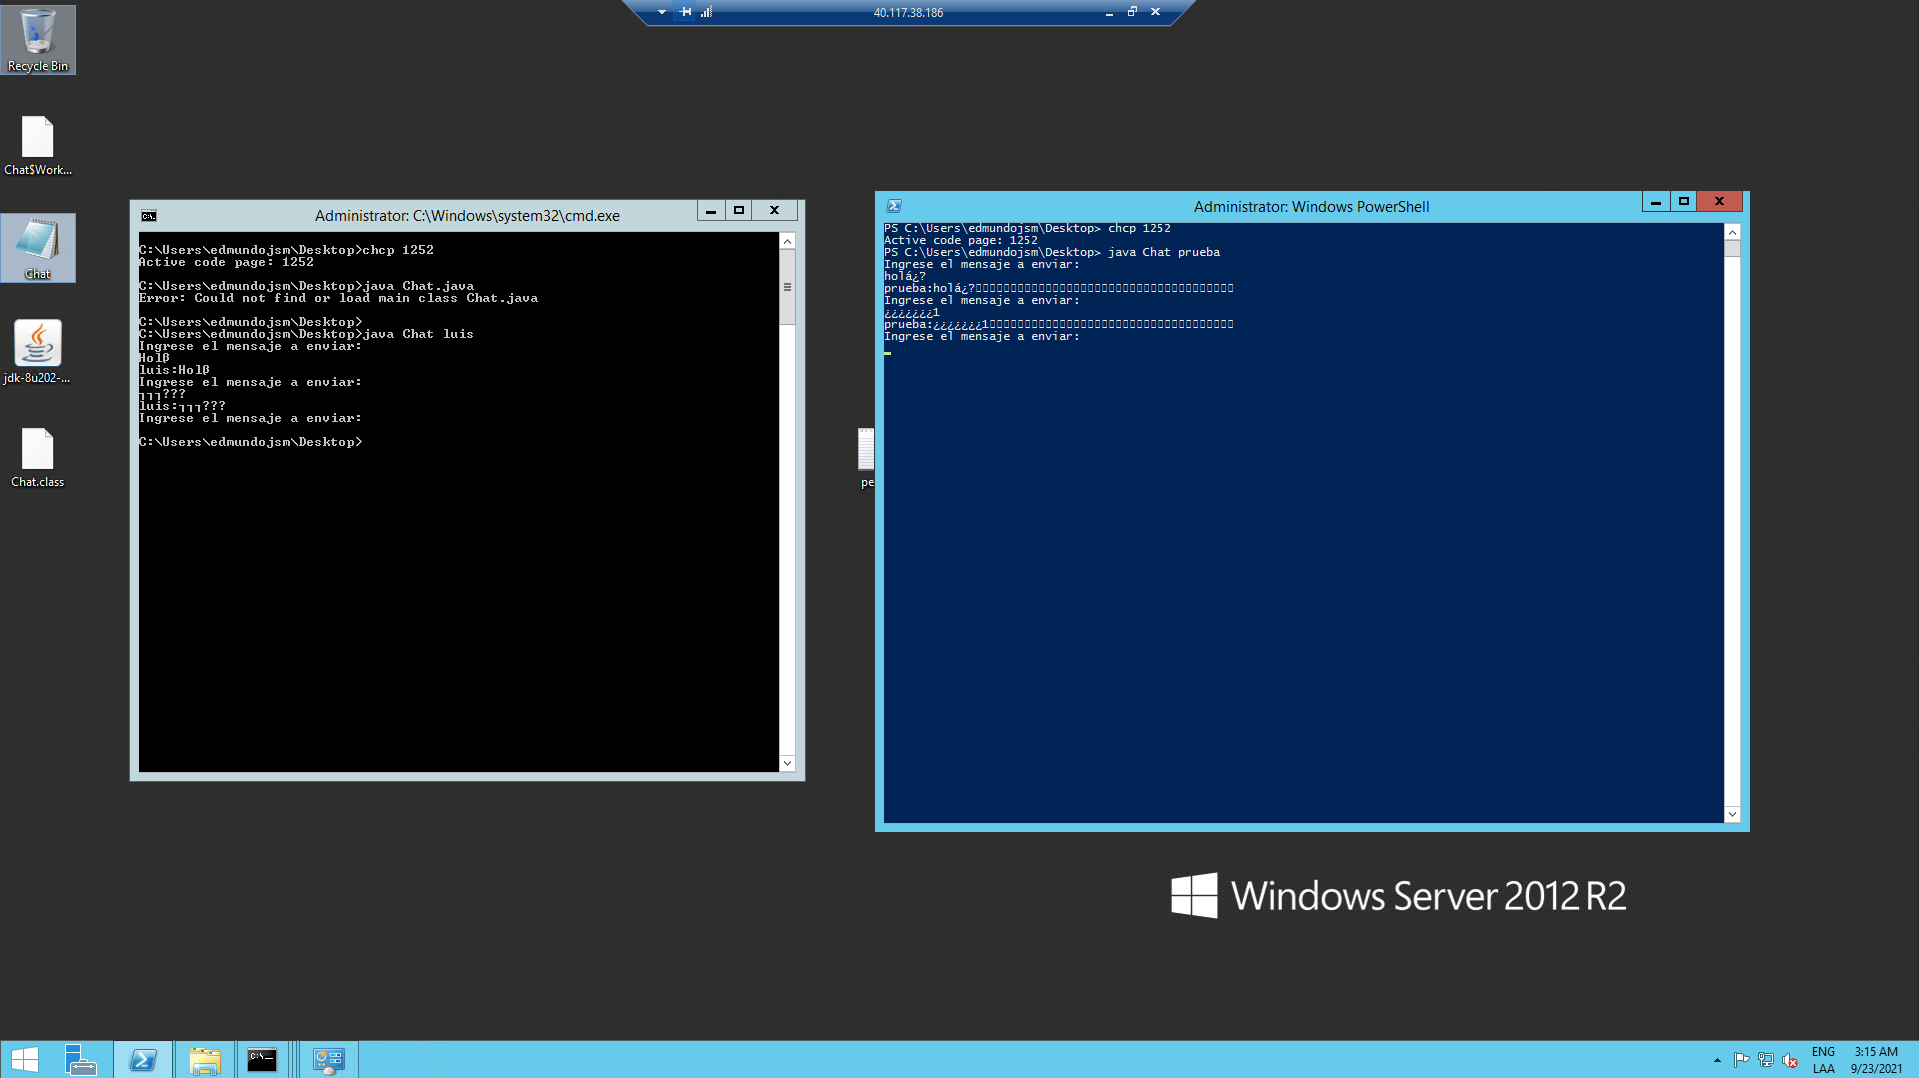
\includegraphics[scale=0.34]{resources/erroreschcp1252.png}
			\caption{Errores usando pagina de código 1252 y UTF8. }\label{fig:picture}
		\end{figure}
		Ahora como vemos en la figura 22 vemos que el código de pagina por defecto de Windows Server 2012 es la 437, al buscar la tabla de caracteres definidos vemos que contiene los caracteres especiales de la practica por lo que en lugar de modificar el código de pagina lo mejor es adaptar el programa.
		\begin{figure}[H]
			\centering
			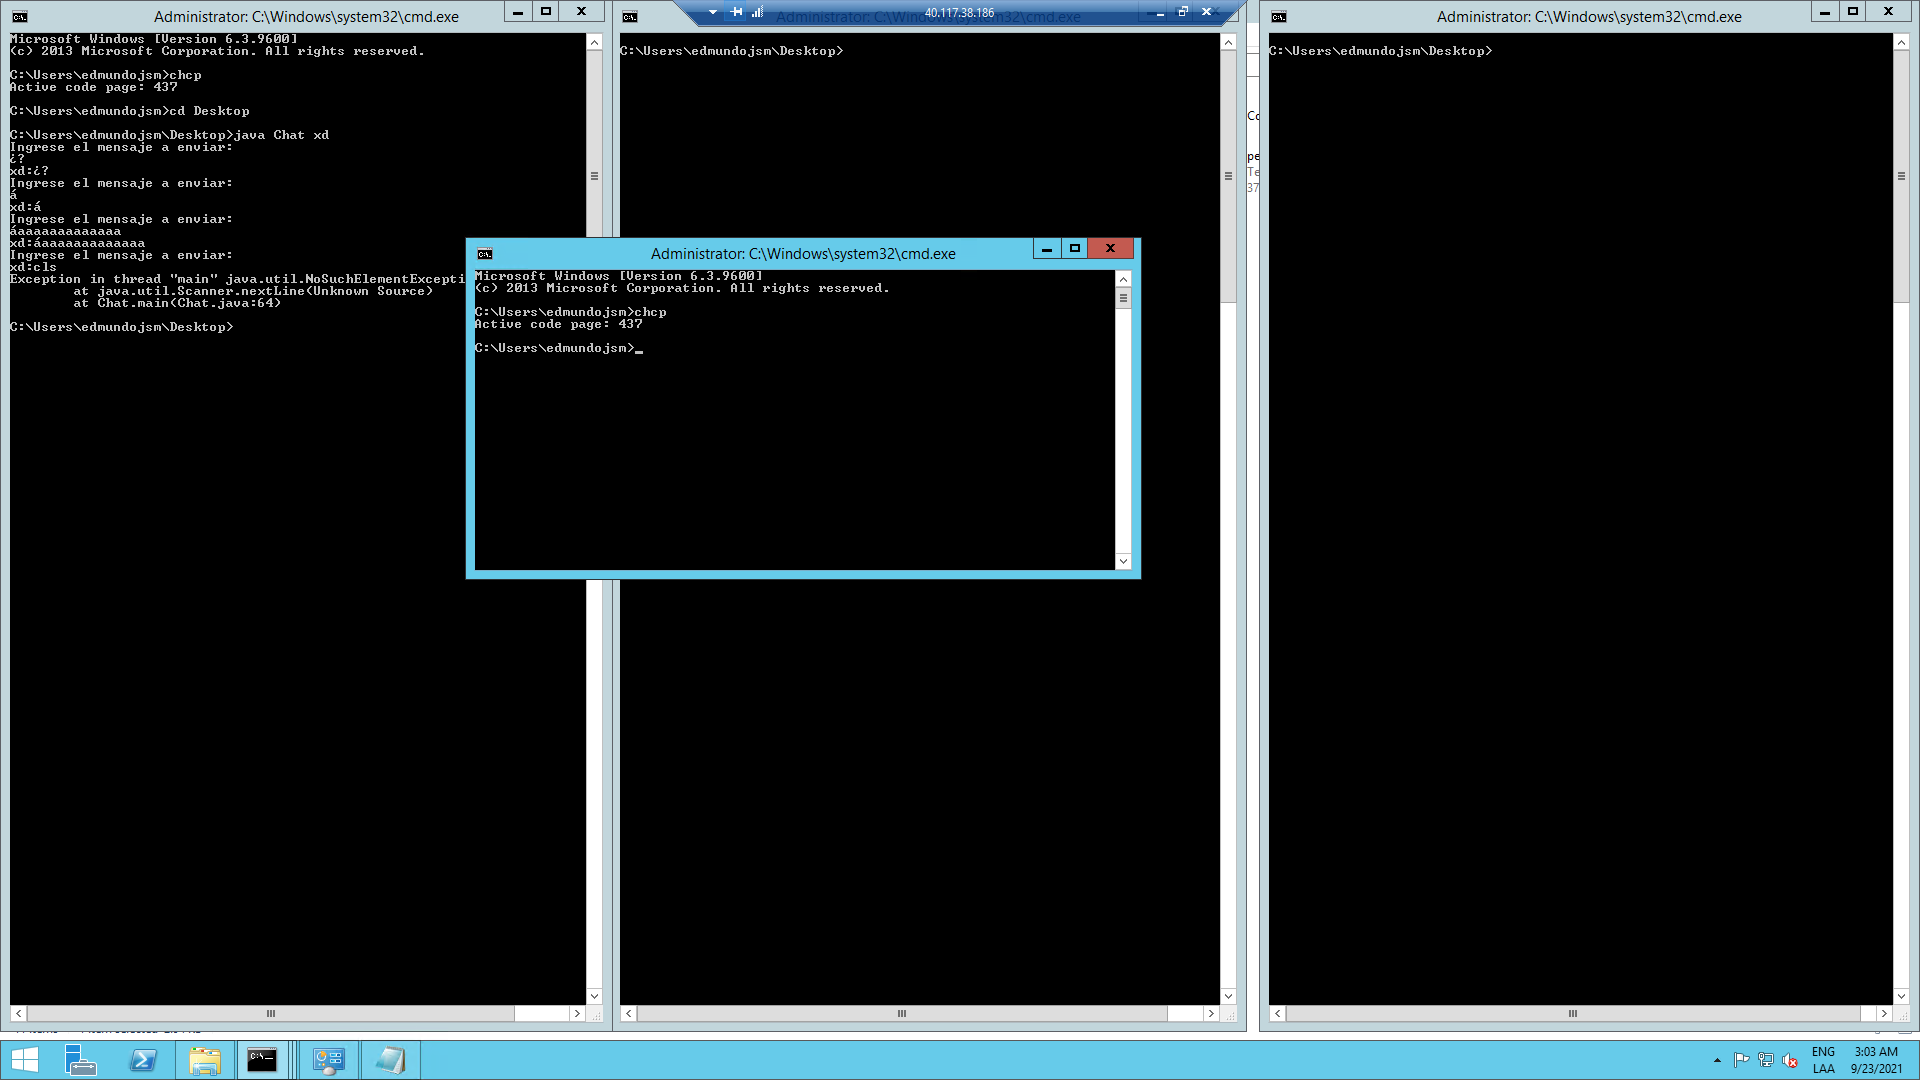
\includegraphics[scale=0.34]{resources/defaultcp.png}
			\caption{Código de pagina por defecto. }\label{fig:picture}
		\end{figure}
		Ahora si en la imagen 23 podemos ver la compilación del archivo Chat.java y que ademas Java esta correctamente instalado en nuestra maquina.
		\begin{figure}[H]
			\centering
			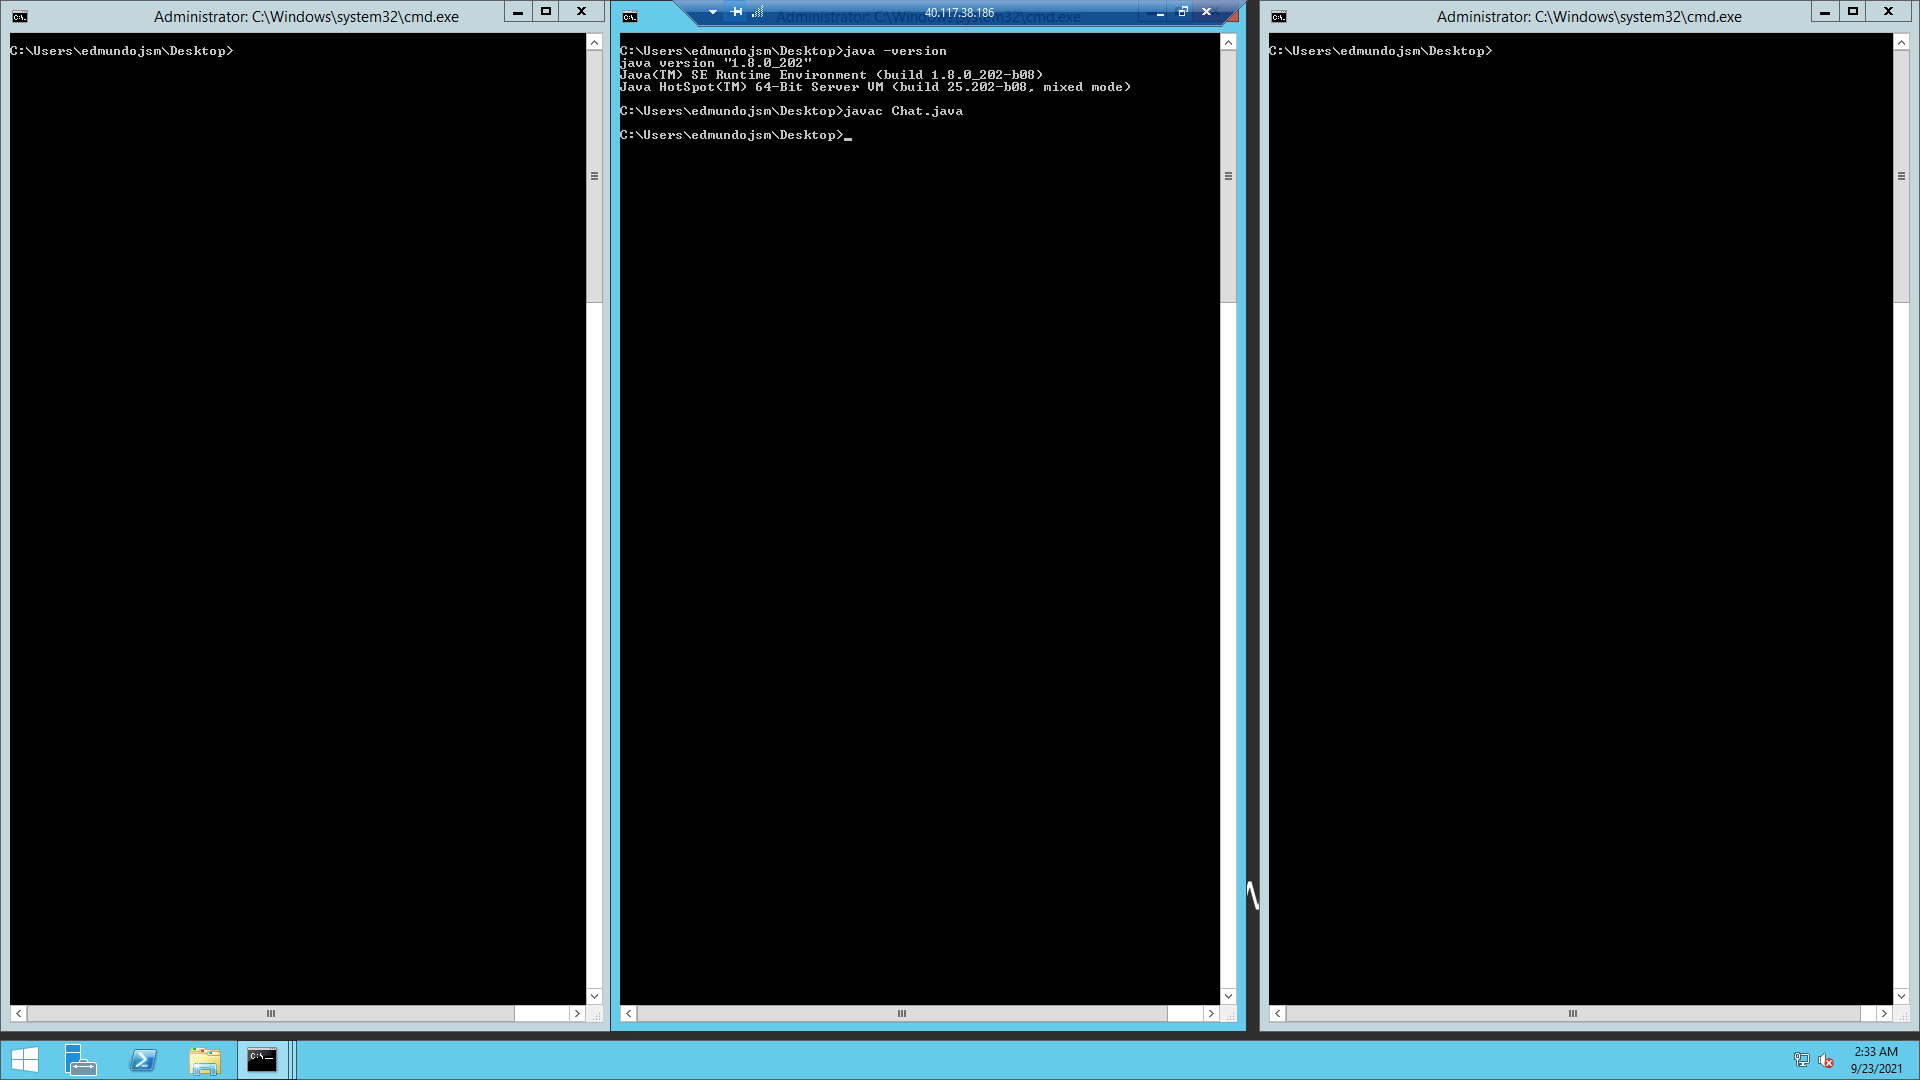
\includegraphics[scale=0.34]{resources/compiliacionyjavabien.png}
			\caption{Compilación e instalación de Java correctas. }\label{fig:picture}
		\end{figure}
		\newpage
		\subsection{Ejecución del programa}
		Una vez compilado nuestro programa se procedió a realizar la conversación solicita, adicional a esto en la misma figura, la cual es la figura 24 podemos ver como también se esta utilizando el código de pagina por defecto.
		\begin{figure}[H]
			\centering
			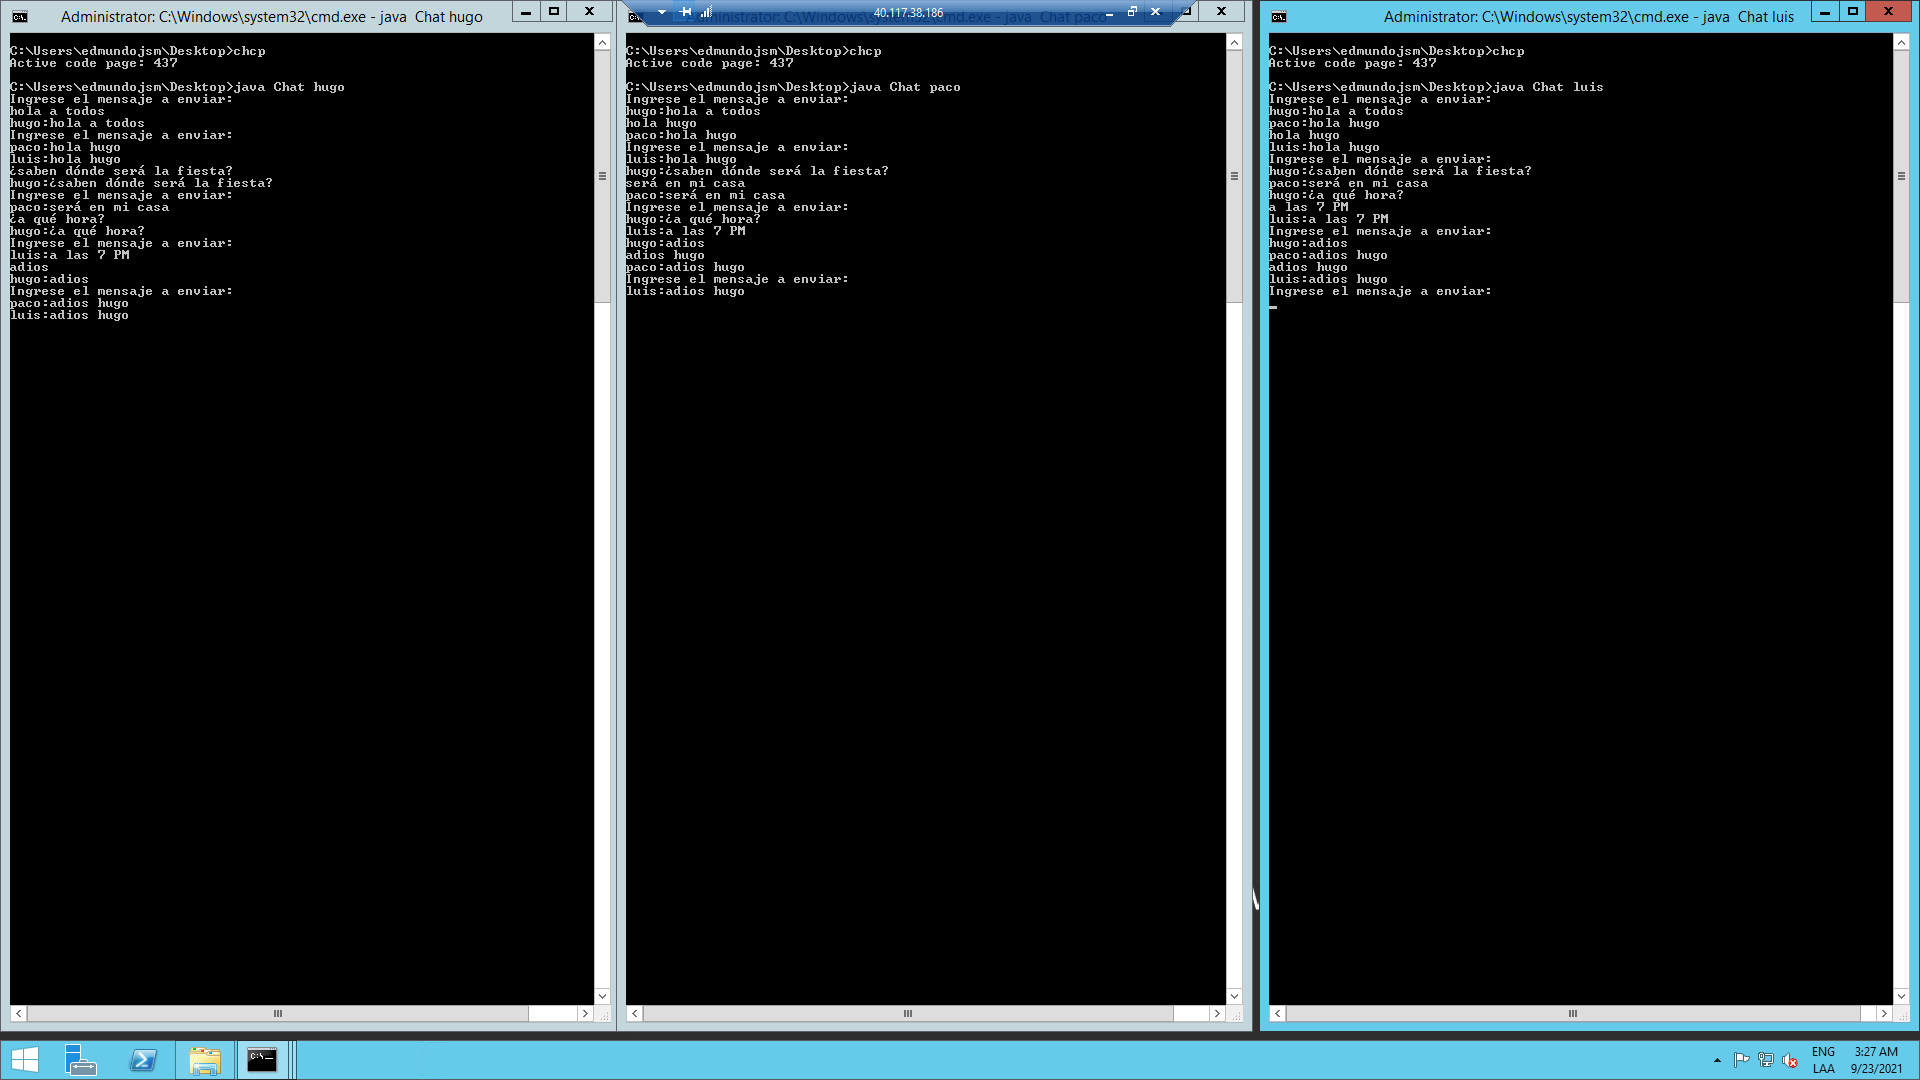
\includegraphics[scale=0.34]{resources/resultadofinal.png}
			\caption{Conversación solicitada y código de pagina utilizado. }\label{fig:picture}
		\end{figure}
	\section{Conclusiones}
	En esta práctica desarrollamos un cliente multicast, pero como se nos menciono en clase el desarrollo de este tipo de servidores es muy sencilla, ya que todos los mensajes que se envían serán recibidos por todos los dispositivos conectados a la misma red y al mismo puerto, realmente no hay mayor problema en el desarrollo del chat. Realmente lo tardo fue lo que vimos a través de este reporte que es el código de pagina y que tipo de codificación le corresponde, también hacer la elección de como leer la entrada del teclado. Finalmente me gustaría recordar que en el archivo comprimido se encuentra el archivo que lleva como nombre Chat.java es el que se uso para realizar la ejecución del programa, sin embargo, también se encuentra un archivo Chatv1.java que es el archivo que se desarrollo primeramente con el uso del código de pagina 1252 y utf8 mencionar que si se quiere usar este archivo se tendrá que modificar el nombre a Chat ya que si no se hace eso el nombre de la clase no coincidirá y Java no nos dejara compilar el archivo.
	\begin{thebibliography}{1}
 \bibitem[label1]{cite_key1} Oracle. n.d. Supported Encodings. [online] Available at: https://docs.oracle.com/javase/8/docs/technotes/guides/intl/encoding.doc.html [Accessed 23 September 2021].
  \bibitem[label1]{cite_key1} Oracle. n.d. Scanner (Java Platform SE 7 ). [online] Available at: https://docs.oracle.com/javase/7/docs/api/java/util/Scanner.html [Accessed 23 September 2021].
  \bibitem[label1]{cite_key1} Es.wikipedia.org. 2020. Windows-1252 - Wikipedia, la enciclopedia libre. [online] Available at: https://es.wikipedia.org/wiki/Windows-1252 [Accessed 23 September 2021].
  \bibitem[label1]{cite_key1} Es.wikipedia.org. 2021. Página de códigos 437 - Wikipedia, la enciclopedia libre. [online] Available at: \url{https://es.wikipedia.org/wiki/P\%C3\%A1gina_de_c\%C3\%B3digos_437} [Accessed 23 September 2021].
  \bibitem[label1]{cite_key1} Es.wikipedia.org. 2020. Página de códigos 850 - Wikipedia, la enciclopedia libre. [online] Available at: \url{https://es.wikipedia.org/wiki/P\%C3\%A1gina_de_c\%C3\%B3digos_850} [Accessed 23 September 2021].
\end{thebibliography}

\end{document}
\end{document}
